% Vorlage für eine Bachelorarbeit
% Siehe auch LaTeX-Kurs von Mathematik-Online
% www.mathematik-online.org/kurse
% Anpassungen für die Fakultät für Mathematik
% am KIT durch Klaus Spitzmüller und Roland Schnaubelt im Dezember 2011

\documentclass[12pt,a4paper]{scrartcl}
% scrartcl ist eine abgeleitete Artikel-Klasse im Koma-Skript
% zur Kontrolle des Umbruchs Klassenoption draft verwenden


% die folgenden Packete erlauben den Gebrauch von Umlauten und ß
% in der Latex Datei
\usepackage[utf8]{inputenc}
% \usepackage[latin1]{inputenc} %  Alternativ unter Windows
\usepackage[T1]{fontenc}
\usepackage[ngerman]{babel}

\usepackage[pdftex]{graphicx}
\usepackage{latexsym}
\usepackage{amsmath,amssymb,amsthm}

\usepackage{csquotes}
\MakeOuterQuote{"}

% Abstand obere Blattkante zur Kopfzeile ist 2.54cm - 15mm
\setlength{\topmargin}{-15mm}


% Umgebungen für Definitionen, Sätze, usw.
% Es werden Sätze, Definitionen etc innerhalb einer Section mit
% 1.1, 1.2 etc durchnummeriert, ebenso die Gleichungen mit (1.1), (1.2) ..

\newtheorem{Satz}{Satz}[section]
\newtheorem{Definition}[Satz]{Definition}     
\newtheorem{Lemma}[Satz]{Lemma}	
                  
\numberwithin{equation}{section} 

% einige Abkuerzungen
\newcommand{\C}{\mathbb{C}} % komplexe
\newcommand{\K}{\mathbb{K}} % komplexe
\newcommand{\R}{\mathbb{R}} % reelle
\newcommand{\Q}{\mathbb{Q}} % rationale
\newcommand{\Z}{\mathbb{Z}} % ganze
\newcommand{\N}{\mathbb{N}} % natuerliche



\begin{document}
  % Keine Seitenzahlen im Vorspann
  \pagestyle{empty}

  % Titelblatt der Arbeit
  \begin{titlepage}

    
\includegraphics[scale=0.45]{kit-logo.jpg}
    \vspace*{2cm} 

 \begin{center} \large 
    
    Masterarbeit
    \vspace*{2cm}

    {\huge Analyse der elektrischen Signale zur Angriffserkennung in industriellen Systemen basierend auf maschinellem Lernen}
    \vspace*{2.5cm}

    Yorick Laly
    \vspace*{1.5cm}

    30/04/2021
    \vspace*{4.5cm}


    Betreuung: Prof. Kristian Kroschel, Prof. Sebastian Randel, M.Sc. Markus Karch, M.Sc. Anne Borcherding, M.Sc. Ankush Meshram \\[0.7cm]
    Fakult\"at für Elektrotechnik und Informationstechnik \\[0.7cm]
		Karlsruher Institut für Technologie
  \end{center}
\end{titlepage}



%%%%%%%%%%%%%%%%%%%%%%%%%%%%%%%%%
 \newpage  % neuer Abschnitt auf neue Seite, kann auch entfallen
%%%%%%%%%%%%%%%%%%%%%%%%%%%%%%%%%
% Ab sofort Seitenzahlen in der Kopfzeile anzeigen
  \pagestyle{headings}

\section*{Erklärung der Selbstständigkeit}



Hiermit versichere ich, dass ich die Arbeit selbständig verfasst habe und keine
anderen als die angegebenen Quellen und Hilfsmittel benutzt habe, die wörtlich
oder inhaltlich übernommenen Stellen als solche kenntlich gemacht habe und die
Satzung des Karlsruher Instituts für Technologie zur Sicherung guter
wissenschaftlicher Praxis in der gültigen Fassung beachtet habe.

\vspace{1cm}

\hspace{5,5cm} Karlsruhe, 30/04/2021 \hspace{0.5cm} \makebox[2in]{\hrulefill}





%%%%%%%%%%%%%%%%%%%%%%%%%%%%%%%%%
 \newpage  % neuer Abschnitt auf neue Seite, kann auch entfallen
%%%%%%%%%%%%%%%%%%%%%%%%%%%%%%%%%
% Ab sofort Seitenzahlen in der Kopfzeile anzeigen
  \pagestyle{headings}

  % Inhaltsverzeichnis
  \tableofcontents


%%%%%%%%%%%%%%%%%%%%%%%%%%%%%%%%%
 \newpage  % neuer Abschnitt auf neue Seite, kann auch entfallen
%%%%%%%%%%%%%%%%%%%%%%%%%%%%%%%%%
% Ab sofort Seitenzahlen in der Kopfzeile anzeigen
\thispagestyle{plain}

\section*{Kurzfassung}

Industrielle Systeme werden zunehmend vernetzt, um die Verwaltung eines gesamten Industriekomplexes, der eine große Anzahl von Maschinen enthalten kann, mithilfe von Computern zu erleichtern. Dies macht sie jedoch angesichts von Computerangriffen, die die im industriellen System vorhandenen Geräte beschädigen können, umso schwächer. Diese Angriffe können erkannt werden, indem die Signale untersucht werden, die direkt von den Prozesssensoren und -aktoren kommen. Da diese Angriffe darauf abzielen, Geräte zu zerstören, indem ihr ursprüngliches Verhalten drastisch geändert wird, können wir diese Verhaltensänderungen erkennen, indem wir die Signale des Prozesses mithilfe von Methoden des maschinellen Lernens untersuchen.

In dieser Masterarbeit wurde ein Prozess untersucht, der Objekte nach ihren Materialien sortiert. Damit habe ich einen Datensatz von über 130 Läufen mit normalem Verhalten aufgezeichnet. Dieser Datensatz wurde halbiert, ein Teil für das Methodentraining und der andere Teil für das Testen. Mit den abgegriffenen Signalen wurde eine Anomalieerkennung unter Verwendung verschiedener maschineller Lernmethoden durchgeführt. Die folgenden Methoden werden verglichen: Convolutionnal Neural Network, Autoencoder, Support Vector Machine, Local Outlier Factor und Density-Based Spatial Clustering of Applications with Noise (DBSCAN). Unter den verschiedenen Methoden ist DBSCAN die Methode mit der wir die besten Ergebnisse für die Erkennung von Anomalien erzielen. 

%%%%%%%%%%%%%%%%%%%%%%%%%%%%%%%%%
 \newpage  % neuer Abschnitt auf neue Seite, kann auch entfallen
%%%%%%%%%%%%%%%%%%%%%%%%%%%%%%%%%

  % Ab sofort Seitenzahlen in der Kopfzeile anzeigen
  \pagestyle{headings}

\section{Einleitung}
Um die Verwaltung von Maschinen in einem industriellen System zu erleichtern, werden zunehmend Computersysteme verwendet, die Informationen zentralisieren, die den Zustand von Maschinen oder Daten von Sensoren und Aktoren an einem oder mehreren zentralen Computern anzeigen. Diese industriellen Systeme sind jedoch ein leichtes Ziel für Cyber-Angriffe, da die in diesen Systemen verwendeten Softwarekomponenten und Netzwerkprotokolle veraltet sind, aber auch, weil sie keine oder nur mangelhafte Verteidigungsmechanismen gegen Computerangriffe haben. Ein Cyber-Angriff auf ein industrielles System kann die Produktionsketten verlangsamen, Geräte zerstören, die sehr teuer sein können, oder sogar das Leben der Arbeiter im Industriekomplex gefährden. Es besteht daher die Notwendigkeit, diese industriellen Systeme zu schützen. 

Ein Cyber-Angriff auf ein industrielles System hat meist das primäre Ziel das Verhalten eines Prozesses innerhalb des industriellen Systems zu ändern. Diese Art von Verhaltensänderung kann durch Untersuchung der Signale von den Prozesssensoren und -aktoren erkannt werden. Diese Verhaltensänderung innerhalb eines Signals von einem Sensor wird als Anomalie bezeichnet. 

Mit dem Aufkommen des maschinellen Lernens sind Methoden entstanden, die Anomalien in Systemen erkennen können. Diese Methoden basieren hauptsächlich auf dem Lernen eines Normalverhaltens. Diese Phase wird als Lernphase bezeichnet. Anschließend wird in die Detektionsphase übergangen. Hierbei wird das das erlernte Normalverhalten mit den aktuell beobachteten Prozessdaten abgeglichen. Tritt eine zu große Abweichung vom erlernten Normalverhalten auf, spricht man vom Auftreten einer Anomalie. 

In dieser Masterarbeit wurde an einem industrielle Modellprozess untersucht, welcher Objekte nach ihrer Beschaffenheiten sortiert, welche Signale aus dem Prozess stammen und ob Anomalien in diesen Signalen durch maschinelles Lernen erkannt werden können. Zunächst mussten die von den verschiedenen Sensoren und Aktoren des Prozesses kommenden Signale abgegriffen werden, um sie anschließend auf einem Computer einlesen zu können. Dann wurden die wiederhergestellten Daten vorbereitet. Verschiedene Methoden des maschinellen Lernens, bei denen Anomalien über neuronale Netze oder Cluster erkannt oder vorhergesagt werden, wurden verglichen, um die Methode zu ermitteln, mit der wir die besten Ergebnisse erzielen. 

%%%%%%%%%%%%%%%%%%%%%%%%%%%%%%%%%
 \newpage  % neuer Abschnitt auf neue Seite, kann auch entfallen
%%%%%%%%%%%%%%%%%%%%%%%%%%%%%%%%%
% Ab sofort Seitenzahlen in der Kopfzeile anzeigen
  \pagestyle{headings}

\section{Grundlagen}

In diesem Teil wird beschrieben, wie industrielle Systeme für Cyber-Angriffe schwach sind und wie sie derzeit vor solchen Angriffen geschützt sind. In diesem Teil wird auch erklärt, wie verschiedene Methoden des maschinellen Lernens funktionieren. 

\subsection{Angriffserkennung in industriellen Netzen}

Um die Verwaltung von Maschinen innerhalb eines Industriekomplexes zu erleichtern, verwenden Unternehmen heutzutage industrielle Systeme, die zunehmend miteinander verbunden sind und zunehmend drahtlose Kommunikation verwenden. Dank dieser Art von Kommunikation ist es viel einfacher, Informationen über den Zustand und den Betrieb von Maschinen zu sammeln, diese aber auch von einem einzigen Computer aus fernzusteuern. Diese Kommunikation verwenden jedoch einfache und bekannte Protokolle wie das Transmission Control Protocol (TCP). Es ist dann für eine externe Person, die mit diesen Arten von Protokollen vertraut ist, einfach, die Kommunikation innerhalb des Systems zu beobachten und sie zu stören, indem beispielsweise die Kommunikation mit einem Teil des Systems blockiert wird. Ein böswilliger Mitarbeiter kann aber auch aus dem Industriekomplex heraus angreifen, indem er eine Maschine manuell sabotiert oder Malware über einen USB-Stick injiziert.

Cyber-Angriffe dieser Art sind bereits aufgetreten, insbesondere im Jahr 2010 während des Cyber-Angriffs Stuxnet auf Nuklearanlagen im Iran. Malware wurde von einem Mitarbeiter über einen USB-Stick injiziert, um Geräte für die Kernforschung zu zerstören. Der Computerwurm replizierte zunächst selbstständig auf den Maschinen\footnotemark{} und analysierte die Kommunikation mit SCADA (Supervisory Control and Data Acquisition) und lokalisierte alle Computergeräte unter Verwendung von Windows als Betriebssystem. Windows ist das von Herstellern am häufigsten verwendeten Betriebssystem und ein leichtes Ziel für Angreifer. Durch Ausnutzen einer Schwachstelle in diesem Betriebssystem konnte der Computerwurm Zugriff auf die speicherprogrammierbare Steuerung (SPS) erhalten. Der Wurm kann daher Codes blockieren, die in die SPS eingegeben werden, und schlechte Informationen an andere Maschinen und IT-Geräte senden. Die Malware könnte auch über USB angeschlossene Geräte infizieren, wodurch sie schnell in den gesamten Industriekomplex eindringen konnte.

\footnotetext{http://large.stanford.edu/courses/2015/ph241/holloway1/}

Ein weiteres neueres Beispiel kam Anfang dieses Jahres mit einem Angriff auf eine Wasseraufbereitungsanlage\footnotemark{} in den Vereinigten Staaten. Eine Person außerhalb dieser Anlage hat es geschafft, die Kontrolle zu übernehmen, indem sie erneut eine Schwachstelle im Windows-Betriebssystem eines der Computer ausnutzte, der den Gehalt an chemischen Elementen im Wasser verwaltet, und diese Rate auf extrem hohe Werte erhöhte. So hoch, dass zu einer Wasservergiftung führte, die gefährlich sein könnte zum Verzehr. Dieses Eindringen konnte jedoch von einem der Mitarbeiter festgestellt werden, der die seltsame Bewegung seines Computerzeigers bemerkte, während sich die Maus nicht bewegte.

\footnotetext{https://www.industrialdefender.com/florida-water-treatment-plant-cyber-attack/}

Diese Vorfälle hatten zur Folgen, dass nun auch vermehrt in industriellen Kontrollsystemen vermehrt Verteidigungsmechanismen eingesetzt werden. Das bekannteste System ist das Network Intrusion Detection System (NIDS). NIDS analysiert eingehende Pakete im Switch und erkennt Kommunikationsstörungen. Das Funktionsprinzip wird in Abbildung 1 dargestellt.

In einem industriellen System übermittelt der Prozess Informationen über den Status seiner Sensoren und Aktoren an den Buskoppler, der die Informationen an speicherprogrammierbare Steuerung (SPS) sendet. Die SPS sendet die Daten an die Switch, der die Daten an eine Firewall und dann an einen Computer zurücksendet.

Während eines Cyber-Angriffs greift der Computerwurm wie Stuxnet oder Irongate hauptsächlich die SPS an, wodurch der Prozess unterbrochen wird, während schlechte Informationen an den Switch gesendet werden. 

\begin{figure}[ht!]
	\centering
	  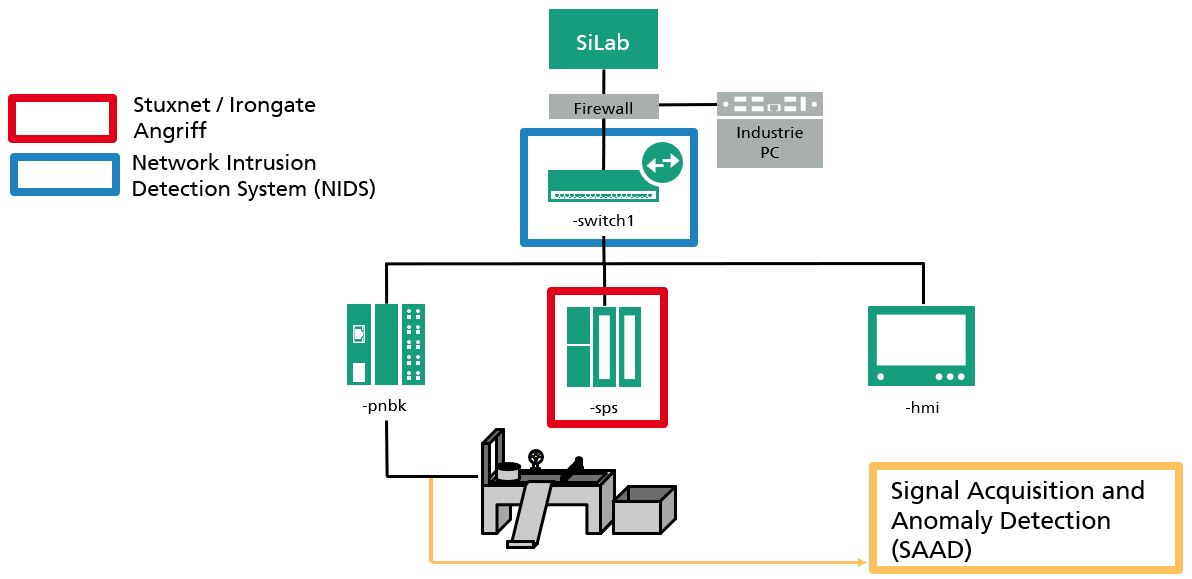
\includegraphics[scale=0.5]{ganze_systeme.jpg}
	  \caption{Industrielle System Beispiel}
\end{figure}


NIDS erkennt die Stuxnet- und Irongate-Angriffe jedoch nicht, da diese Angriffe auf der SPS auftreten und sie daher die Kontrolle über den Prozess übernehmen können, während sie dem Switch und anderen Komponenten falsche Informationen über den Status des Prozesses senden.

Um das Verhalten des Prozesses auch in solchen Angriffszenarien beobachten zu können, werden in dieser Arbeit die analogen Signale der Sensoren und Aktoren direkt am Ausgang des Prozesses analysiert. Diese Signale geben Auskunft über das Verhalten des Prozesses in Echtzeit. Dank des im Rahmen dieser Masterarbeit entwickelten Systems namens Signal Acquisition and Anomaly Detection (SAAD) im Verhalten des Prozesses. Auf diese Weise kann SAAD jede Verhaltensänderung unabhängig vom industriellen System, seinen Komponenten, dem den Prozess steuernden Computer, der Software und dem verwendeten Betriebssystem erkennen.

\subsection{Convolutionnal Neural Network}

Das Convolutional Neural Network (CNN) ist eine Methode, die auf neuronalen Netzen und Faltung basiert, um Muster in Signalen oder Bildern zu lernen. Während eines CNN wird der Wert jedes Punktes der nächsten Schicht aus den benachbarten Werten dieses Punktes der vorherigen Schicht berechnet. Diese Operation wird durch die Abbildung \ref{conv} dargestellt.

\begin{figure}[ht!]
	\centering
	  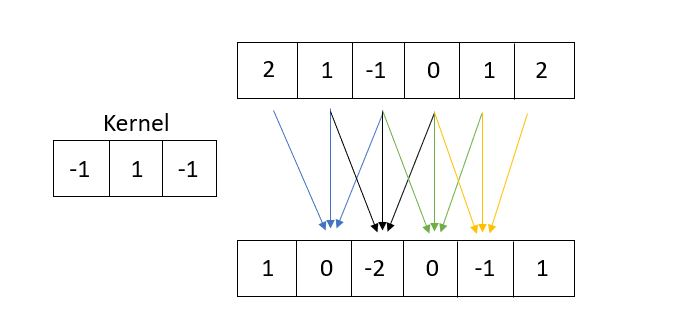
\includegraphics[scale=0.6]{conv.jpg}
	  \caption{Faltung Beispiel}
	\label{conv}
\end{figure}

Wenn wir zum Beispiel einen Kernel $[-1,1, -1]$ betrachten, ist der Wert des $i$-ten Punktes des Signales $s$:
 $s_{i-1} * (- 1) + s_{i} + s_{i + 1} * (- 1)$ .

Die Werte des Kernels ändern sich natürlich während des Trainings, um die Kostenfunktion zu reduzieren.

\subsection{Autoencoder}

Der Autoencoder ist ein neuronales Netzwerk, zur Dimensionsreduktion. Der Autoencoder kann neben Dimensionsreduktion auch zur Anomalieerkennung verwendet werden. Jede Schicht wird mit der Funktion "Vollständig verbundene Schicht" mit der nächsten verbunden, d.h. jedes Neuron einer Schicht wird an alle anderen Neuronen der nächsten Schicht weitergeleitet, wie in Abbildung \ref{autoencoder} gezeigt.

Das Autoencoder-Modell besteht aus zwei Teilen, einem Encoder-Teil und einem Decoder-Teil. Der Encoder-Teil besteht darin, die Dimension der Daten zu reduzieren, um die möglichen Rauschen dort zu filtern und die Muster der Signale des normalen Verhaltens zu lernen. Der Decoder-Teil besteht darin, die Daten aus den im Bottleneck vorhandenen Daten, d.h. der Schicht mit der kleinsten Dimension, wiederherzustellen. 


\begin{figure}[ht!]
	\centering
	  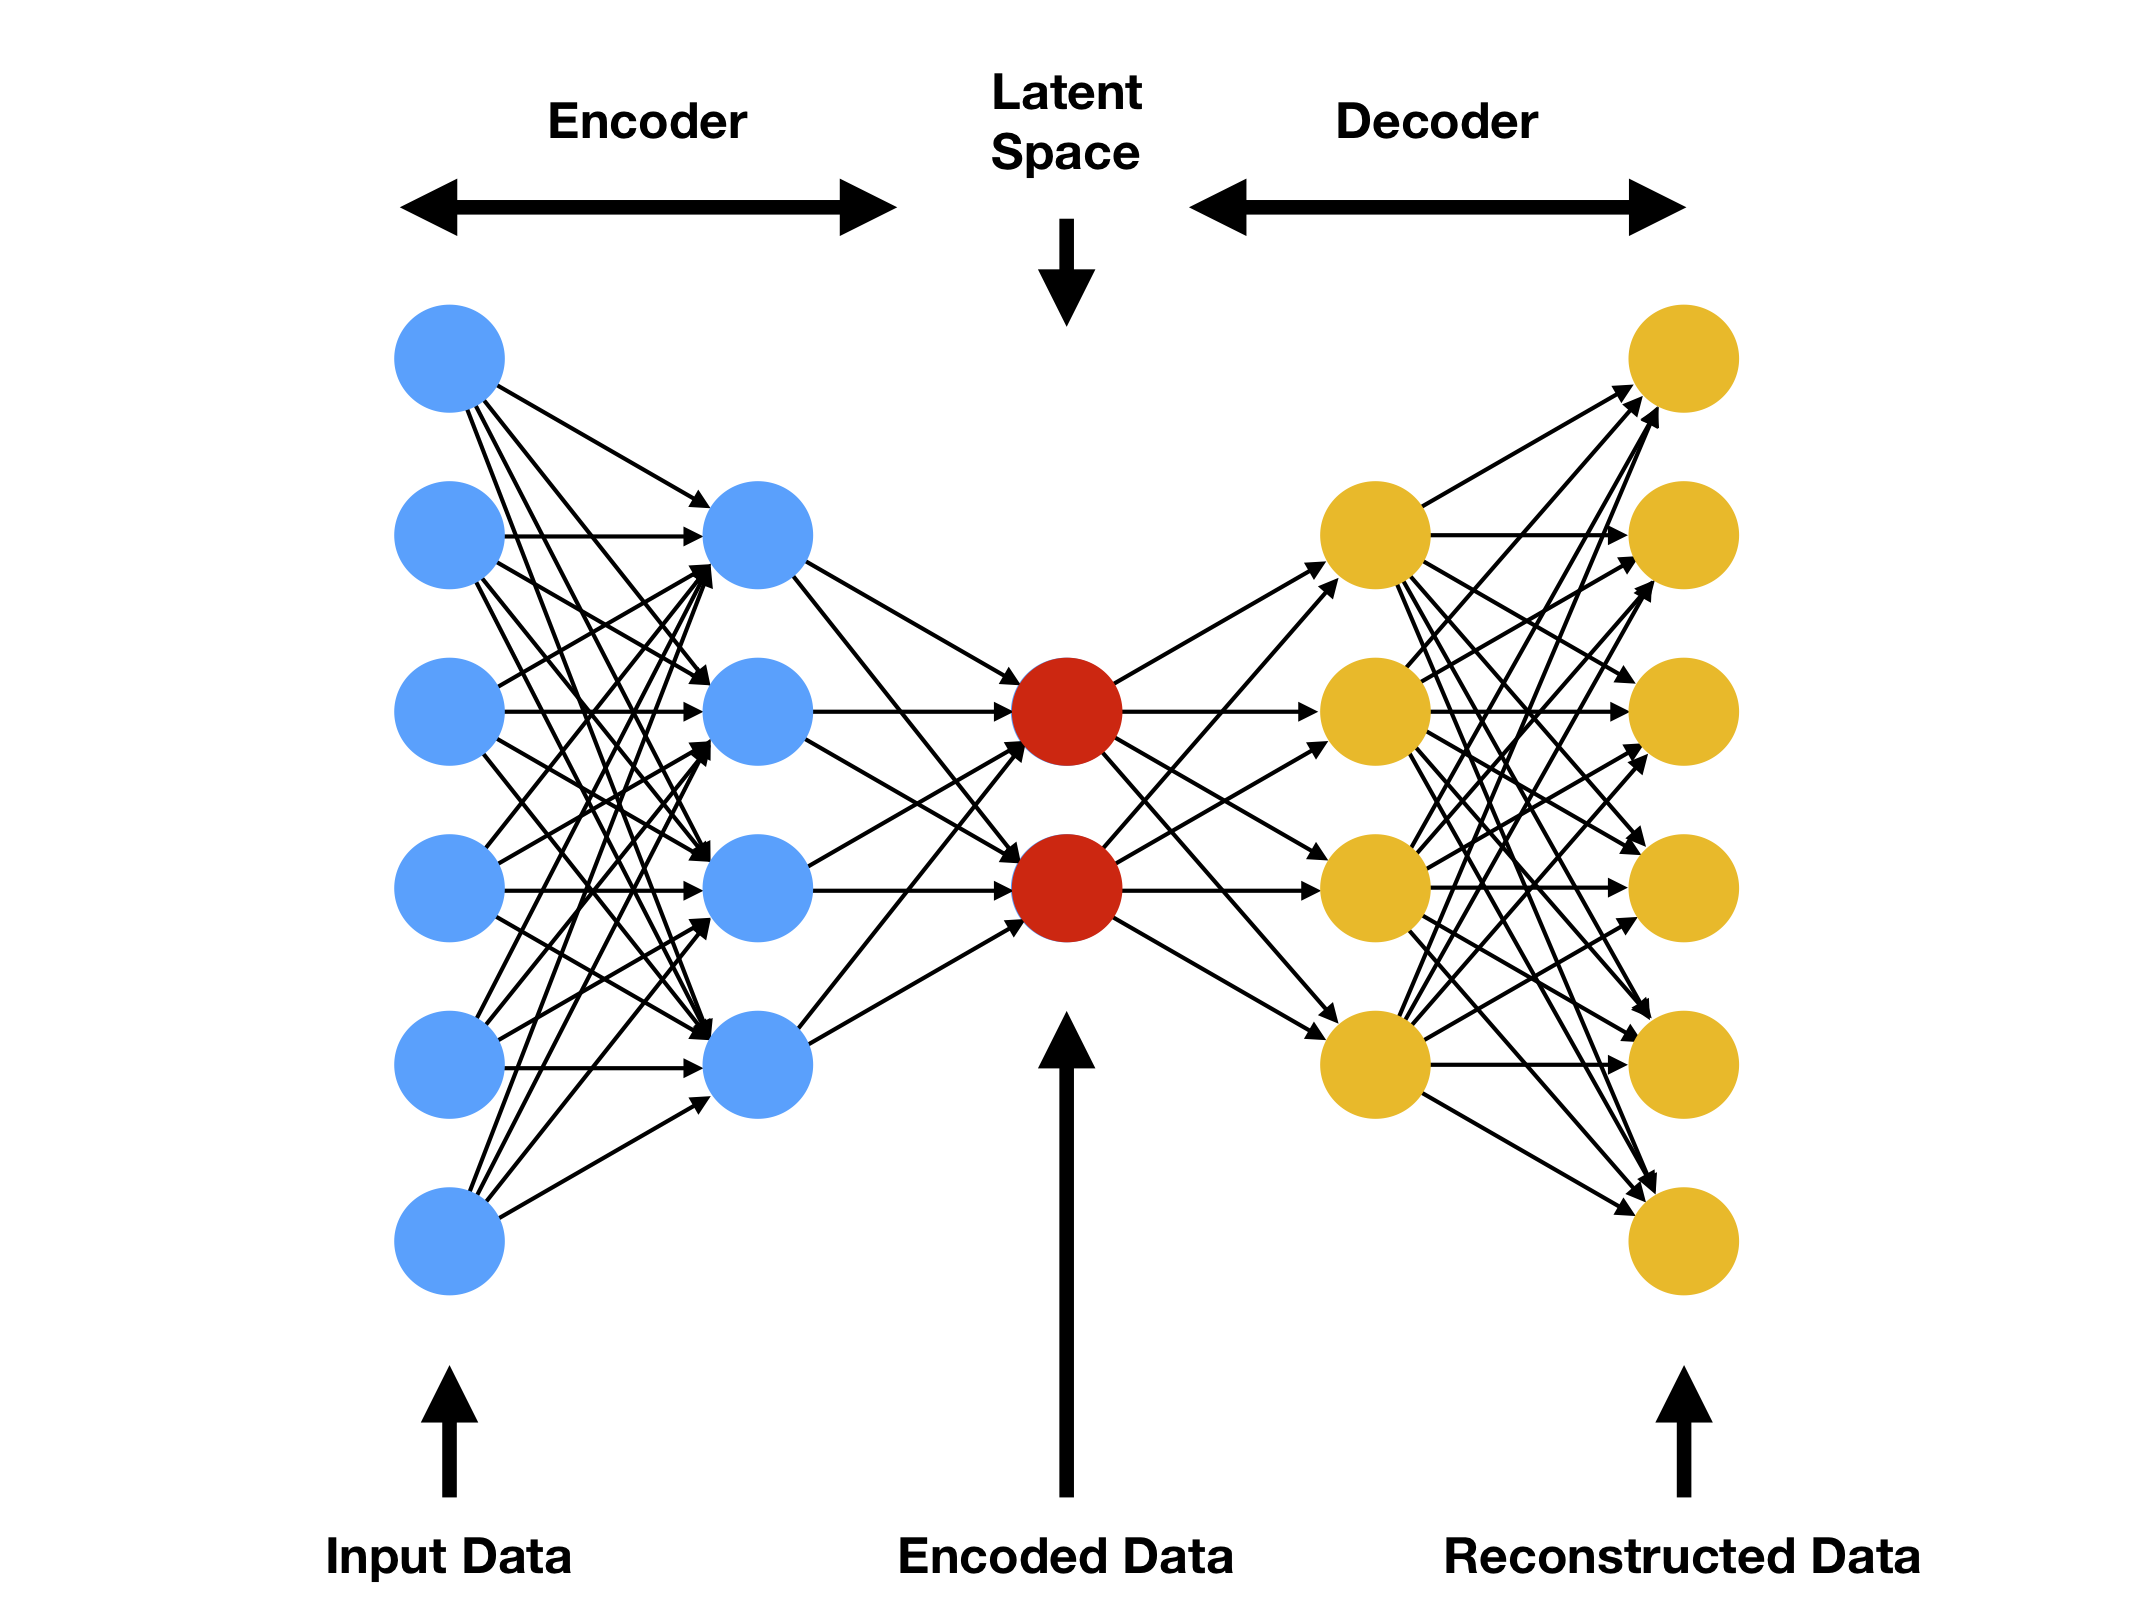
\includegraphics[scale=0.11]{autoencoder.png}
	  \caption[Autoencoder Beispiel]{Autoencoder Beispiel\footnotemark}
	\label{autoencoder}
\end{figure}

\footnotetext{https://miro.medium.com/max/4266/1*QEmCZtruuWwtEOUzew2D4A.png}

\subsection{One Class Support Vector Machine}

Die SVM-Methode (Support Vector Machine) war ursprünglich eine Methode zum Klassifizieren von Daten. Es basiert auf der Erstellung mehrerer Hyperebenen, mit denen die Daten klassifiziert werden. Im Bereich der Anomalieerkennung wird eine einzelne Hyperebene erstellt, in der alle Daten, die Normalwerte eines Systems widerspiegeln, dort gruppiert sind. Die Werte außerhalb dieser Hyperebene sind die Ausreißer, d.h. die Anomalien, die man erkennen möchte. Das Funktionsprinzip wird in Abbildung \ref{SVM} dargestellt. Diese auf einer einzelnen Hyperebene basierende Methode wird als One Class Support Vector Machine bezeichnet. Im Rest dieses Berichts wird diese Arbeit auf die One Class Support Vector Machine-Methode mit dem einfachen Akronym SVM verweisen. 

\footnotetext{https://miro.medium.com/max/4266/1*QEmCZtruuWwtEOUzew2D4A.png}

\begin{figure}[ht!]
	\centering
	  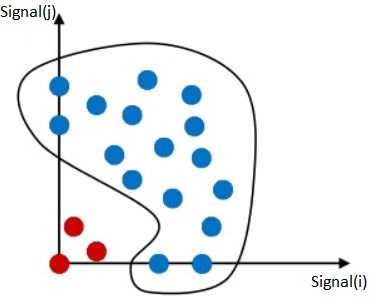
\includegraphics[scale=0.75]{svm.jpg}
	  \caption[SVM Beispiel]{SVM Beispiel\footnote}
	  \label{SVM}
\end{figure}

\footnotetext{https://image.slidesharecdn.com/defense-140531154639-phpapp02/95/machine-learning-challenges-for-automated-prompting-in-smart-homes-33-638.jpg?cb=1401552182}

\subsection{Local Outlier Factor}

Die LOF-Methode (Local Outlier Factor) ist eine Klassifizierungsmethode, die auf der lokalen Dichte eines Objekts basiert und die Anzahl der Nachbarn dieses Punkts in einem Radius um diesen vordefinierten Punkt darstellt. Je höher die Dichte eines Objekts ist, desto mehr Nachbarn gibt es. Dies bedeutet also, dass dieses Objekt zu einer bestimmten Klasse gehört. Das Funktionsprinzip wird in Abbildung \ref{LOF} dargestellt. Im Fall der Erkennungsanomalie befinden sich idealerweise alle Objekte, die das normale Verhalten des Systems darstellen, in einer einzigen Klasse mit hoher Dichte, und alle anderen Punkte mit niedrigerer Dichte sind die Ausreißer, die gesuchten Anomalien. 

\begin{figure}[ht!]
	\centering
	  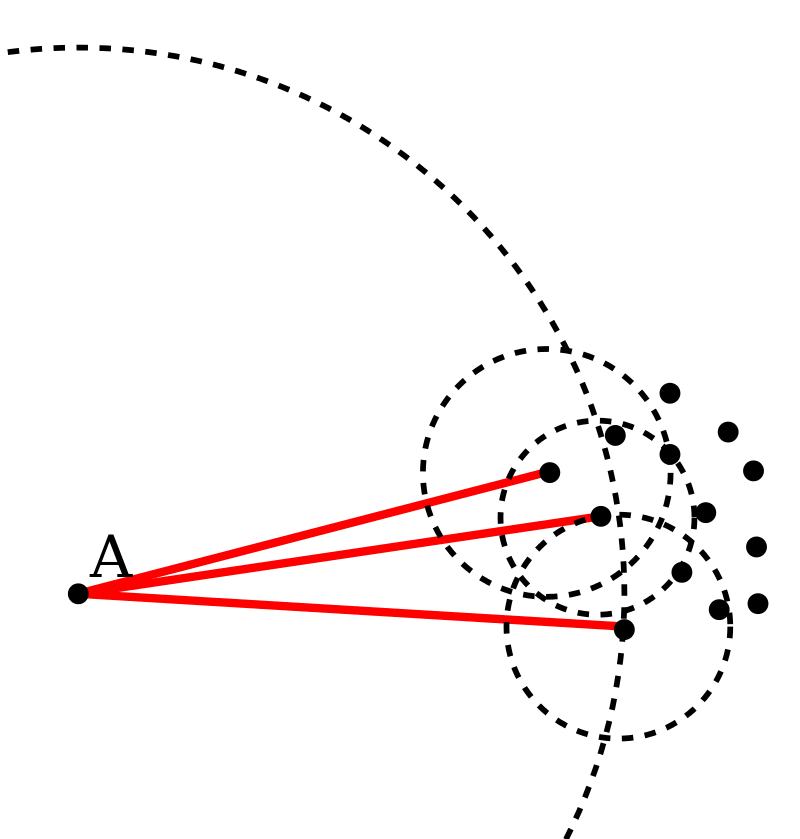
\includegraphics[scale=0.2]{lof.png}
	  \caption[LOF Beispiel]{LOF Beispiel\footnote}
	  \label{LOF}
\end{figure}


\subsection{Density-Based Spatial Clustering of Applications with Noise}

Die Density-Based Spatial Clustering of Applications with Noise (DBSCAN) ähnelt der LOF-Methode, mit der Ausnahme, dass der Benutzer mit DBSCAN nicht nur die Anzahl der Punkte um eine Probe auswählen kann, die als Cluster betrachtet werden sollen, sondern auch den Abstand zwischen den Proben. Das Funktionsprinzip wird in Abbildung \ref{DBSCAN} dargestellt.



\footnotetext{https://upload.wikimedia.org/wikipedia/commons/4/4e/LOF-idea.svg}

\begin{figure}[ht!]
	\centering
	  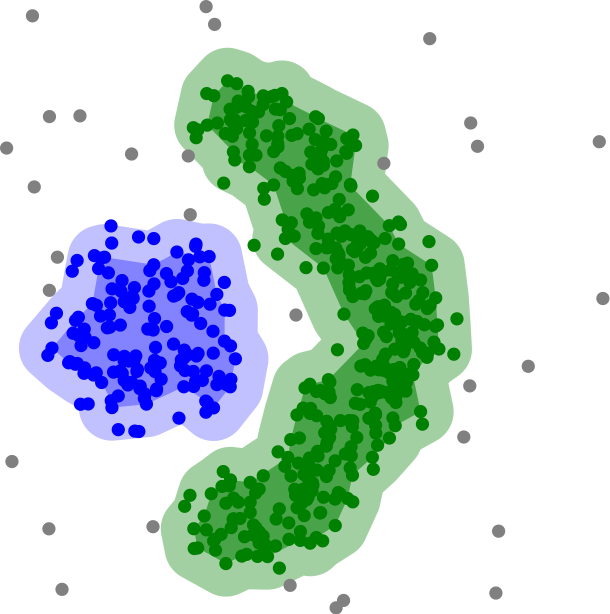
\includegraphics[scale=0.2]{dbscan.png}
	  \caption[DBSCAN Beispiel]{DBSCAN Beispiel\footnote}
	  \label{DBSCAN}
\end{figure}

\footnotetext{https://upload.wikimedia.org/wikipedia/commons/thumb/0/05/DBSCAN-density-data.svg/220px-DBSCAN-density-data.svg.png}

Bei der Anomalieerkennung gruppieren die Cluster das normale Verhalten der Signale und alle Punkte außerhalb der Cluster werden als Anomalien betrachtet. 

Die hier erläuterten Methoden werden als Modell für die Erkennung von Anomalien und normalem Verhalten verwendet. Diese Modelle werden auf unterschiedliche Weise parametrisiert, um ihre Ergebnisse zu optimieren. 

%%%%%%%%%%%%%%%%%%%%%%%%%%%%%%%%%
 \newpage  % neuer Abschnitt auf neue Seite, kann auch entfallen
%%%%%%%%%%%%%%%%%%%%%%%%%%%%%%%%%
\section{Verwandte Arbeit}

Die Erkennung von Anomalien erfolgt in dieser Masterarbeit durch Erlernen des normalen Verhaltens durch maschinelles Lernen. In den letzten Jahren hat maschinelles Lernen gezeigt, dass es möglich ist, Muster in Bildern zu erkennen, beispielsweise Objekte oder Gesichter zu erkennen oder Anomalien in elektrischen Signalen mithilfe von Erfahrung aus maschinellem Lernen zu erkennen. Deep-Learning-Methoden sind derzeit die Methoden, die die beste Leistung für die Musterextraktion bieten [1]. 

Diese Arbeit hat mehrere Methoden ausgewählt, die auf unüberwachten Lernen basieren, da es den Vorteil hat, dass es einfacher zu implementieren ist als überwachtes Lernen. Methoden, die unüberwachtes Lernen verwenden, haben auch gezeigt, dass sie flexibel lernen können und daher für jede Art von Prozess verwendet werden können.

Diese Methoden lassen sich nach [2] in zwei Klassen unterteilen: Clustering und Vorhersage basierend auf Zeitreihen. Clustering-Typ-Methoden erstellen einen Cluster, in dem theoretisch die Daten des normalen Verhaltens des Prozesses enthalten sind. Die Daten außerhalb des Clusters sind die Anomalien. Die Methoden vom Typ Vorhersage basierend auf Zeitreihen sagen die nächsten Werte der Signale aus den zuvor erhaltenen Werten vorher. 

\subsection{Convolutionnal Neural Network}

CNN kann sowohl zum Clustering als auch zur Vorhersage verwendet werden. In dieser Masterarbeit wird das neuronale Netzwerk aus [3] implementiert und evaluiert, das ihre Methode zur Vorhersage verwendet. In [3] verwenden sie ein CNN, das aus 5 Faltungsschichten mit einem Kern der Größe 3 und einem Kern der Größe 1 besteht. Das neuronale Netzwerk ist in Abbildung \ref{1DCNN_struktur} dargestellt.

\begin{figure}[h]
	\centering
	  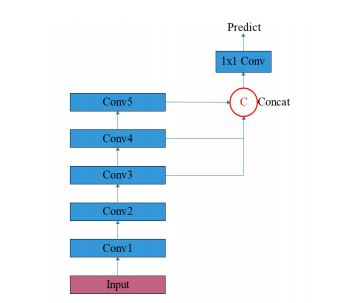
\includegraphics[scale=1]{1DCNN.jpg}
	  \caption{1D-CNN Struktur}
	 \label{1DCNN_struktur}
\end{figure}

Die Schichten 3, 4 und 5 sind verkettet, um eine Overfitting des neuronalen Netzwerks zu verhindern.
Bei der Eingabe des neuronalen Netzwerks werden die Zeitreihen vom Zeitpunkt t bis t + T-1 jedes Sensors und Aktors injiziert, und bei der Ausgabe haben wir die Vorhersage von Zeitreihen vom Zeitpunkt t + T bis t + 2-1 für jeden Sensoren und Aktoren. Die Ausgabe wird mit den wahren Werten der Zeitreihen verglichen. Die Kostenfunktion wird anhand des mittleren quadratischen Fehlers (MSE) berechnet. Mit dieser Methode wurde eine Anomalie Precision zwischen 80 und 95 Prozent erzielt, jedoch mit niedrigen Recall zwischen 10 und 30 Prozent. 

\subsection{Autoencoder}

Der Autoencoder ist ein Modell, mit dem bei der Fehlererkennung sehr gute Ergebnisse erzielt werden können. Es wurde gezeigt, dass mit dem Sparse Autoencoder gute Ergebnisse erzielt werden können [4]. In dieser Masterarbeit wird ein Deep Autoencoder-Modell ohne Sparsity-Kriterium untersucht. Die verwendete Autoencoder-Struktur ist wie in [5] mit 9 vollständig verbundenen Schichten mit der Neuronananzahl 256, 196, 136, 76 und 14. Das Funktionsprinzip ist in Abbildung \ref{auto} dargestellt.


\begin{figure}[h]
	\centering
	  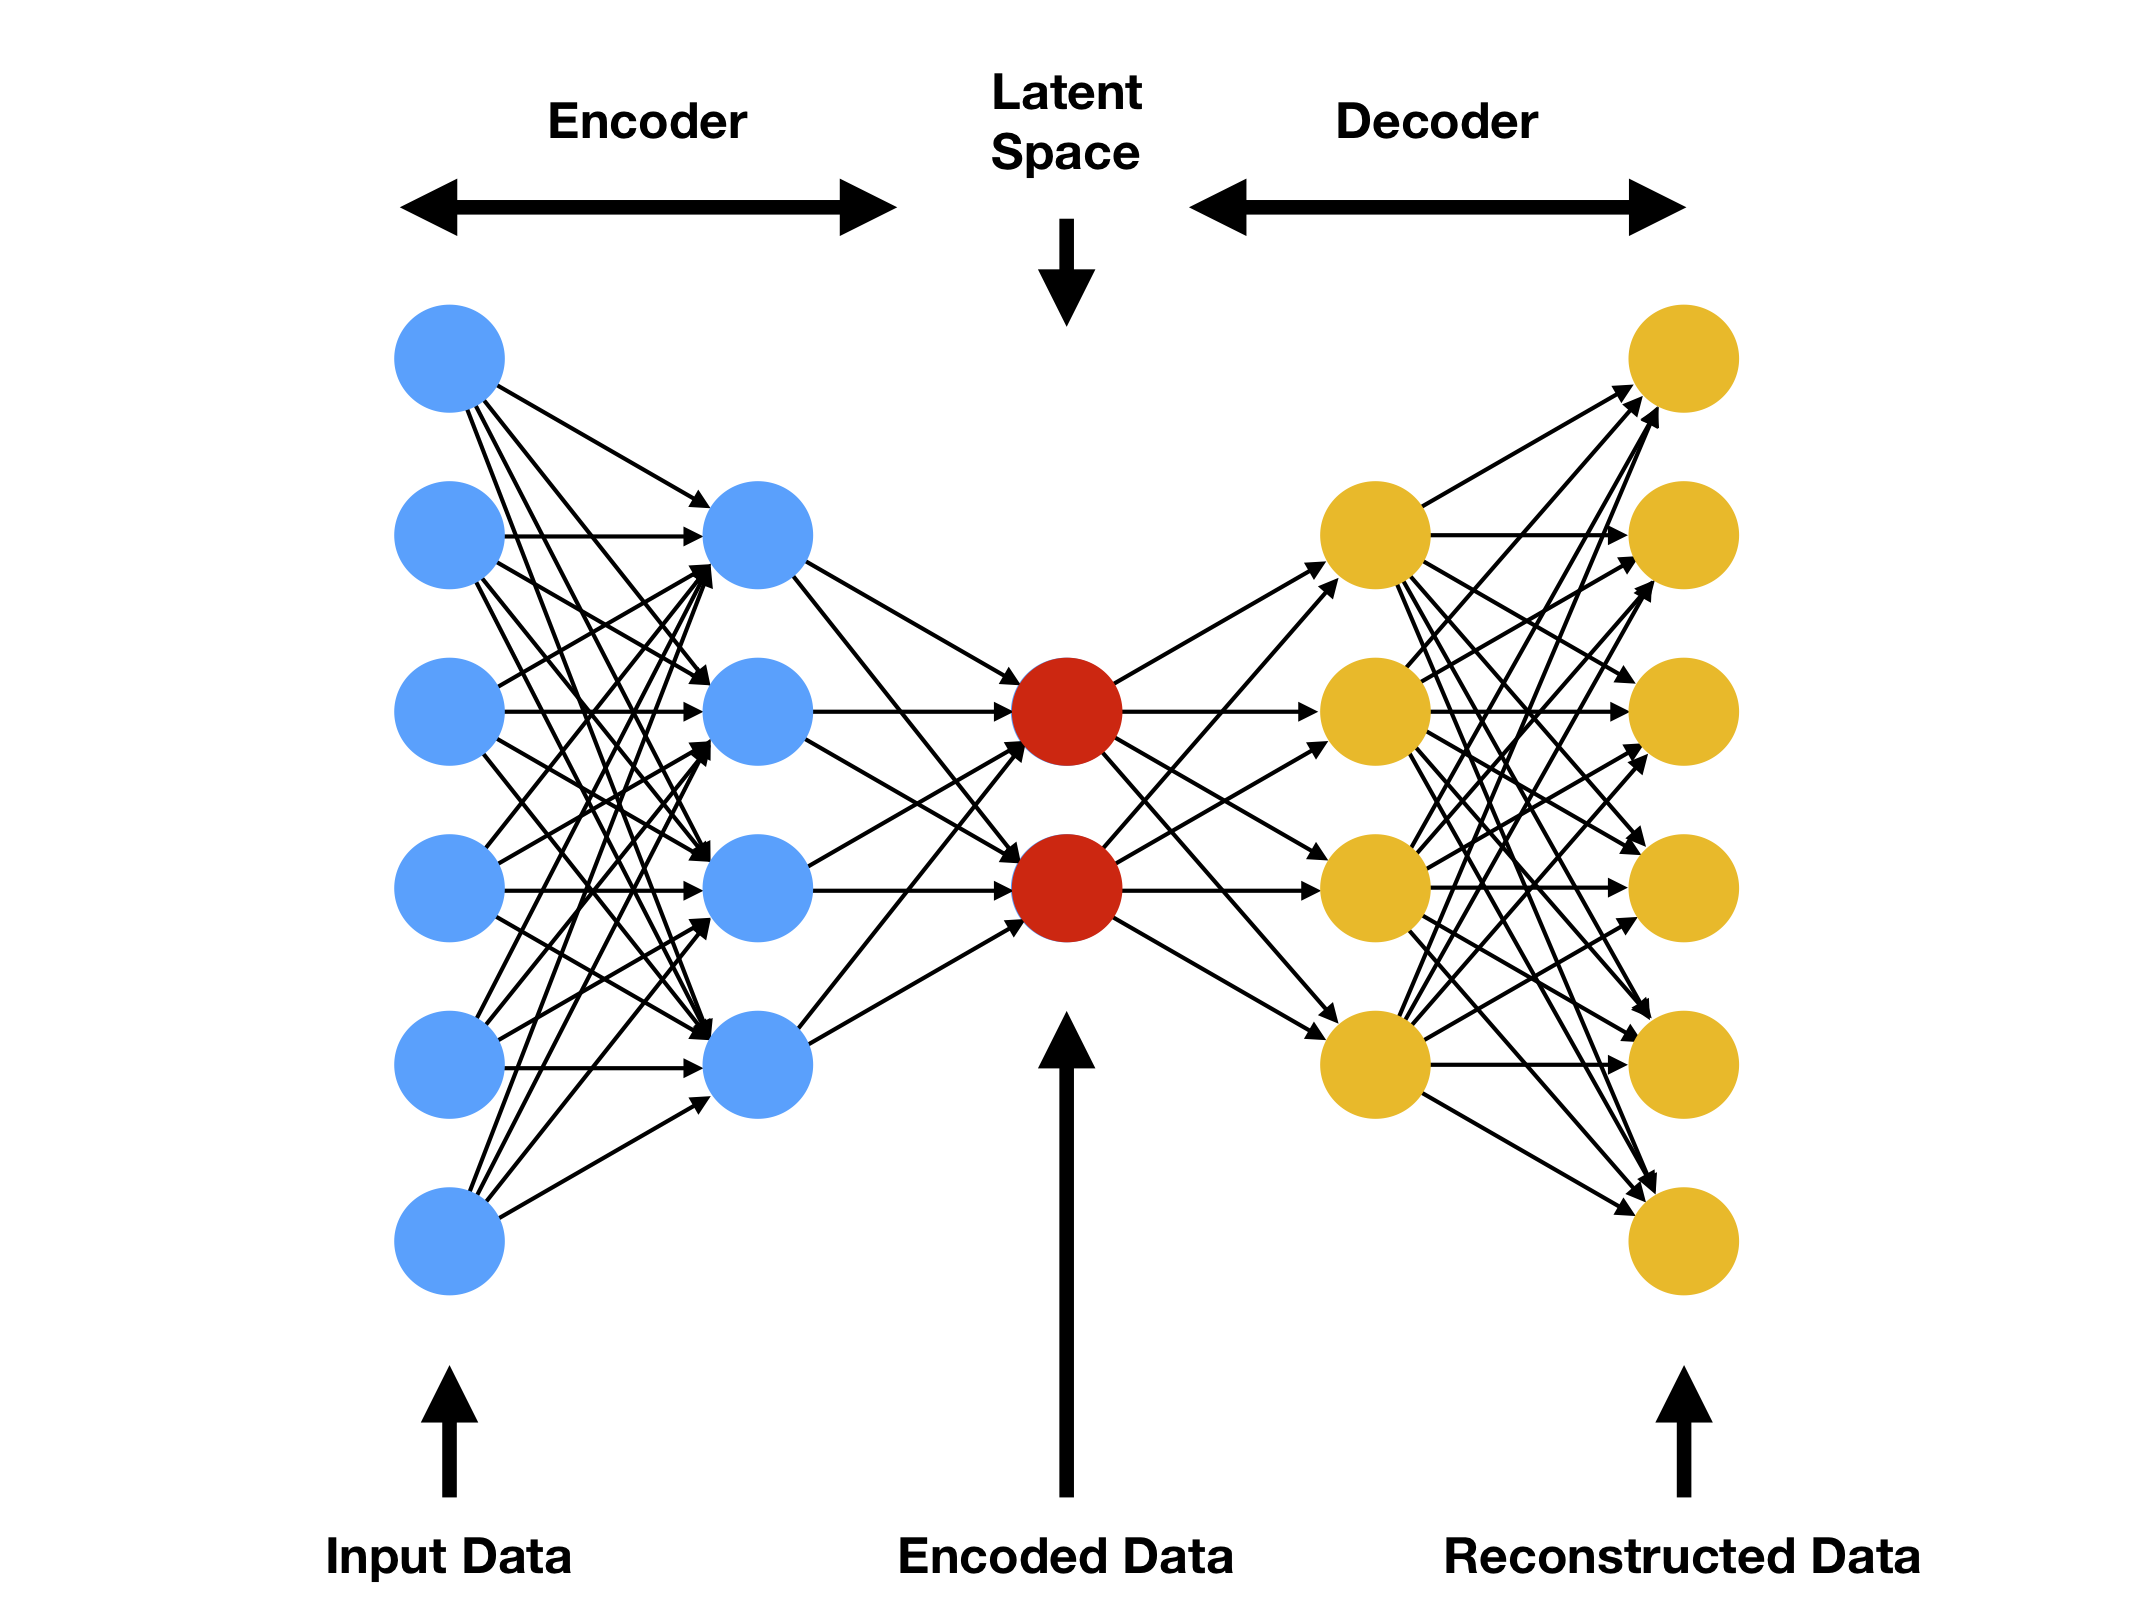
\includegraphics[scale=0.5]{autoencoder.jpg}
	  \caption{Autoencoder mit 9 Schichten}
	\label{auto}
\end{figure}

Als Eingabe für den Autoencoder senden wir für jeden Sensor ein Fenster mit 40 Werten. Der Autoencoder versucht, diese Fenster wiederherzustellen. Die Kostenfunktion wird anhand des mittleren quadratischen Fehlers berechnet. Ein Schwellenwert wird auf den durchschnittlichen Normal Root Mean Square (NRMS) Fehler angewendet und erreicht eine Anomalieerkennungsrate von 97,8 Genauigkeit. 



\subsection{One Class Support Vector Machine}

Die Erkennung von Anomalien in einem industriellen System unter Verwendung der Support Vector Machine wird bereits mit der Vorhersage der Remaining Useful Life (RUL) untersucht [6]. In dieser Studie werden die Leistung einer Maschine und die Vorhersage von Anomalien durch Berechnung der Wahrscheinlichkeit eines Fehlers in der RUL untersucht. 
Im Rahmen dieser Masterarbeit wird eine Implementation der SVM-Methode wiederverwendet, welche ursprünglich zur Aufdeckung von betrügerischen Kreditkarten eingesetzt wird [7]. Hierbei versucht der Autor, betrügerische Kreditkarten in einer Datenbank zu entdecken, die eine große Menge an Kreditkarteninformationen enthält. Da die Erstellung von Daten für Kreditkarten mathematische Funktionen verwendet und nicht zufällig ist, können wir diese Daten untersuchen und ein Muster bestimmen, das echten Kreditkarten gemeinsam ist. Gefälschte Kreditkarten, die diese mathematischen Funktionen nicht verwenden, berücksichtigen daher nicht dieselben Muster und können daher mithilfe einer clusterbasierten Methode erkannt werden. Die Genauigkeit bei der Erkennung der Ausreißer erreicht 91 Prozent. 

Daher können wir diese Arbeit mit der Erkennung von Anomalien in industriellen Systemen parallelisieren, da die Signale von den Sensoren immer die gleichen Muster aufweisen. Dies nennen wir das normale Verhalten des Prozesses und die Anomalien, die wir erkennen möchten, sind einfach Abweichungen von diesem Mustern.  

\subsection{Local Outlier Factor}

Für die LOF-Methode wurde der Ansatz aus [7] genutzt. Daten, die echte Kreditkarten enthalten, werden mit Daten von betrügerischen Kreditkarten verkettet. Die Daten werden an die LOF-Methode übergeben, wobei als Parameter eine Anzahl von Nachbarn gleich 20 ist. Die Evaluation erfolgt durch einfaches Vergleichen jedes Werts des Arrays am Ausgang von LOF mit den Werten der Ground\_truth. Die Accuracy erreicht 89 Prozent. Statt der Erkennung von gefälschten Kreditkarten, handelt es sich bei den hier detektierten Abweichungen um Anomalien in einem industriellen Prozess.  

\subsection{Density-Based Spatial Clustering of Applications with Noise}

Für die DBSCAN-Methode stütze diese Arbeit auch auf die von [7]. Die Daten werden zunächst mit dem StandardScaler vorbereitet. Wie bei der LOF-Methode werden die Daten von echten und gefälschten Kreditkarten zusammen an den DBSCAN gesendet. Die Accuracy bei der Erkennung des Normalverhaltens erreicht 99 Prozent und bei der Erkennung der Anomalie 0 Prozent. Ebenso werde ich versuchen, Anomalien zu erkennen, genau wie in diesem Artikel gefälschte Kreditkarten entdeckt werden. 

%%%%%%%%%%%%%%%%%%%%%%%%%%%%%%%%%
 \newpage  % neuer Abschnitt auf neue Seite, kann auch entfallen
%%%%%%%%%%%%%%%%%%%%%%%%%%%%%%%%%
\section{Signalverarbeitung}

In diesem Teil werden wir zunächst über den Prozess sprechen, bei dem die Anomalieerkennung durchgeführt wird, und über deren Funktionsprinzip. Anschließend wird erklärt, wie der Abgriff der Signale erfolgt ist. Schließlich werden wir die Signale des Prozesses analysieren. 

\subsection{Prozess}

Bei der in dieser Masterarbeit zu untersuchende industrielle Prozess handelt es sich um einen Modellprozess vom Fraunhofer IOSB in Karlsruhe, welcher Objekte (im folgenden auch als Töpfe bezeichnet) nach ihrer Beschaffenheit sortiert. Das komplette System wird in Abbildung \ref{ganze_prozess} dargestellt.

\begin{figure}[h]
	\centering
	  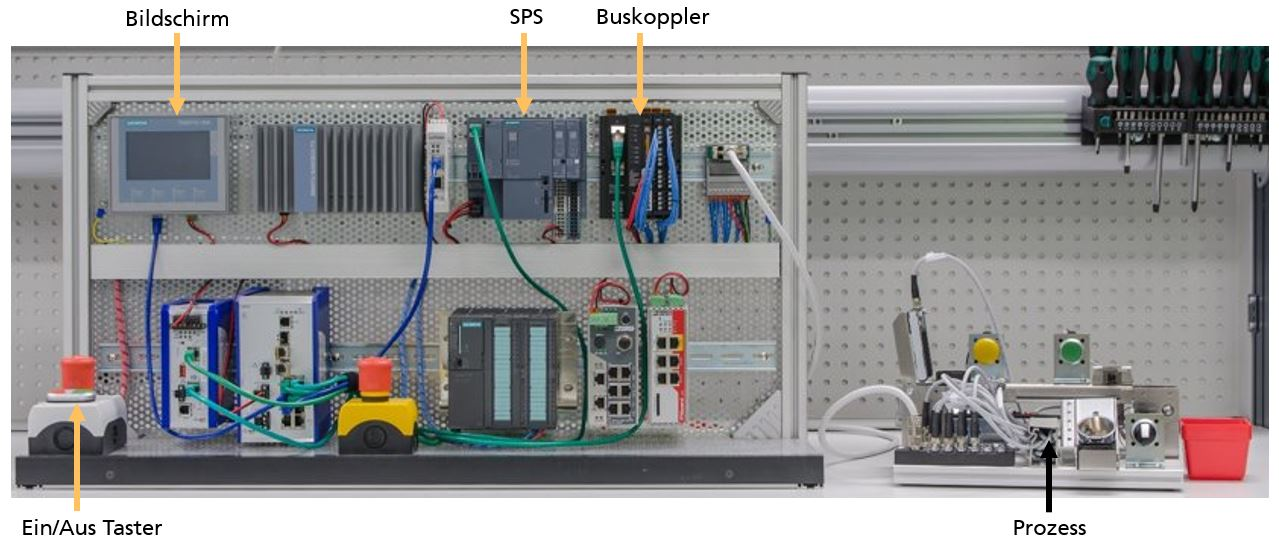
\includegraphics[scale=0.5]{ganze_prozess.jpg}
	  \caption{Komplettsystem}
	\label{ganze_prozess}
\end{figure}


Das gesamte System enthält wie bereits in Abschnitt 1 dargestellt eine SPS, die über den Buskoppler mit dem Prozess kommuniziert. Die SPS ist mit dem Switch verbunden, der Informationen an den Bildschirm sendet. Der Switch wird auch verwendet, um einen Laptop anzuschließen, welcher Cyber-Angriffe durchführen kann.

\vspace*{0.5 cm}

Der Prozess ist einfach und umfasst verschiedene Elemente: eine Lichtschranke, die erkennt, wann ein Objekt durch sie geht, einen induktiven Sensor, der die Beschaffenheit des Objekts erkennt, ein Laufband, der in beide Richtungen (links oder rechts) gehen kann, eine Taster der das Laufband nach links bewegt, eine Schranke, einen Ein / Aus-Schalter und eine Lampe, die blinkt, wenn der Prozess eingeschaltet ist, und eingeschaltet bleibt, wenn der Prozess aktiviert wird. Das Funktionsprinzip wird in Abbildung \ref{prozess_allein} dargestellt.


\begin{figure}[ht!]
	\centering
	  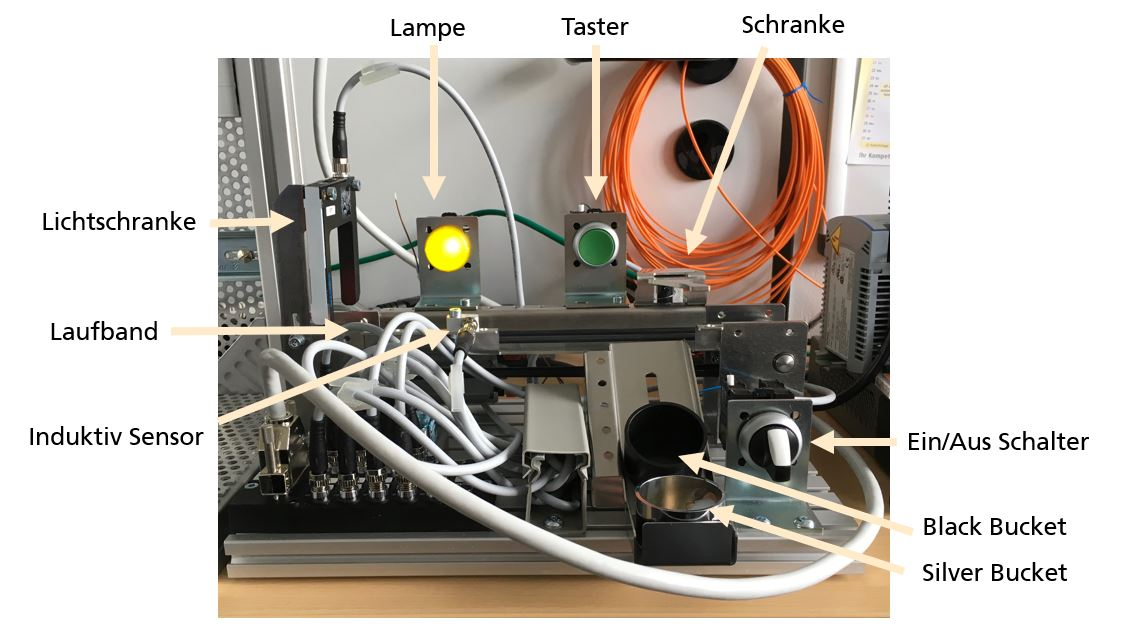
\includegraphics[scale=0.45]{prozess_allein.jpg}
	  \caption{Prozess}
	\label{prozess_allein}
\end{figure}


Der Prozess hat vier normale Verhalten. Der erste ist, wenn der Not-aus Taster gedrückt wird, sollte der Prozess gestoppt werden. Das zweite ist, wenn der Taster gedrückt wird, sollte sich das Laufband nach links bewegen. Die letzte beiden Verhalten treten auf, wenn man einen Topf in der Lichtschranke steckt. Wenn der Topf silbern ist, rollt das Laufband nach rechts, die Lampe bleibt an, der induktive Sensor erkennt den silbernen Topf und die Schranke geht runter. Wenn der Topf schwarz ist, ist das Verhalten dasselbe, außer dass der schwarze Topf vom induktiven Sensor nicht erkannt wird und daher die Schranke nicht runter geht. Das Funktionsprinzip wird in Abbildung \ref{fonctionnement} dargestellt.



Diesen Verhalten werden von verschiedenen maschinellen Lernen Methoden gelernt. Damit können wir eine Anomalie mit Vergleichung des Outputs die Methoden erkennen.

\begin{figure}[ht!]
	\centering
	  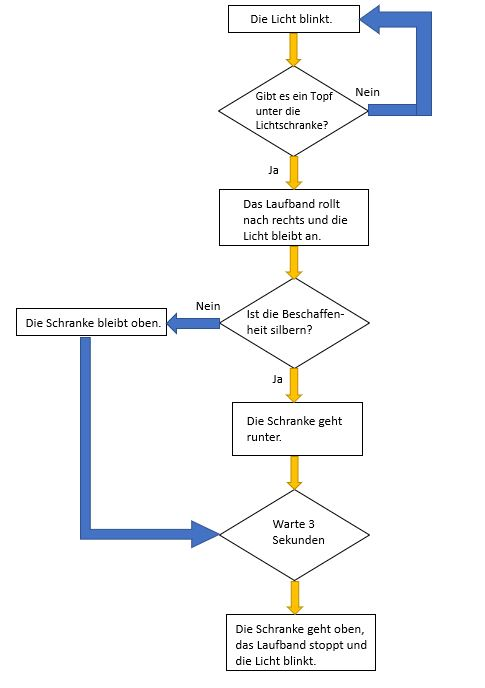
\includegraphics[scale=0.85]{fonctionnement.jpg}
	  \caption{Prozess}
	\label{fonctionnement}
\end{figure}

\subsection{Hardware}

Der Prozess kommuniziert mit dem Rest des Systems über ein DB15-Kabel, das auch als Stromversorgung für den Prozess dient. Der Prozess wird mit 24V betrieben. Um die in den Prozess eintretenden und aus dem Prozess austretenden Signale wiederherstellen zu können, ohne das System und den Prozess zu stören, wurde das einzelne DB 15-Kabel durch einen Y-Schalter und ein Paar DB 15-Kabel ersetzt. Bei einem dritten Kabel können die Signale aus Prozess und System gelesen werden. Das Funktionsprinzip wird durch die Abbildung \ref{yswitch} dargestellt.

\begin{figure}[ht!]
	\centering
	  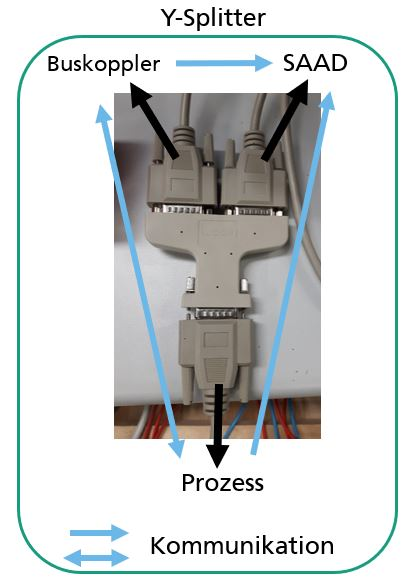
\includegraphics[scale=0.45]{y-switch.jpg}
	  \caption{Y-Switch}
	\label{yswitch}
\end{figure}

Um den Y-Switch mit dem Rest des Systems verbinden zu können, mussten eigene DB15-Stecker-Stecker- und DB15-Buchsen-Buchsen-Kabel hergestellt werden, da es kein solches Kabel auf dem Markt gibt. Also wurden zwei DB15-Stecker-Buchse-Kabel durchgetrennt, um die männlichen und weiblichen Teile miteinander zu löten. Die Abbildung \ref{kabel} zeigt die Drähte, die in den DB15-Kabeln verlötet sind. 

\begin{figure}[ht!]
	\centering
	  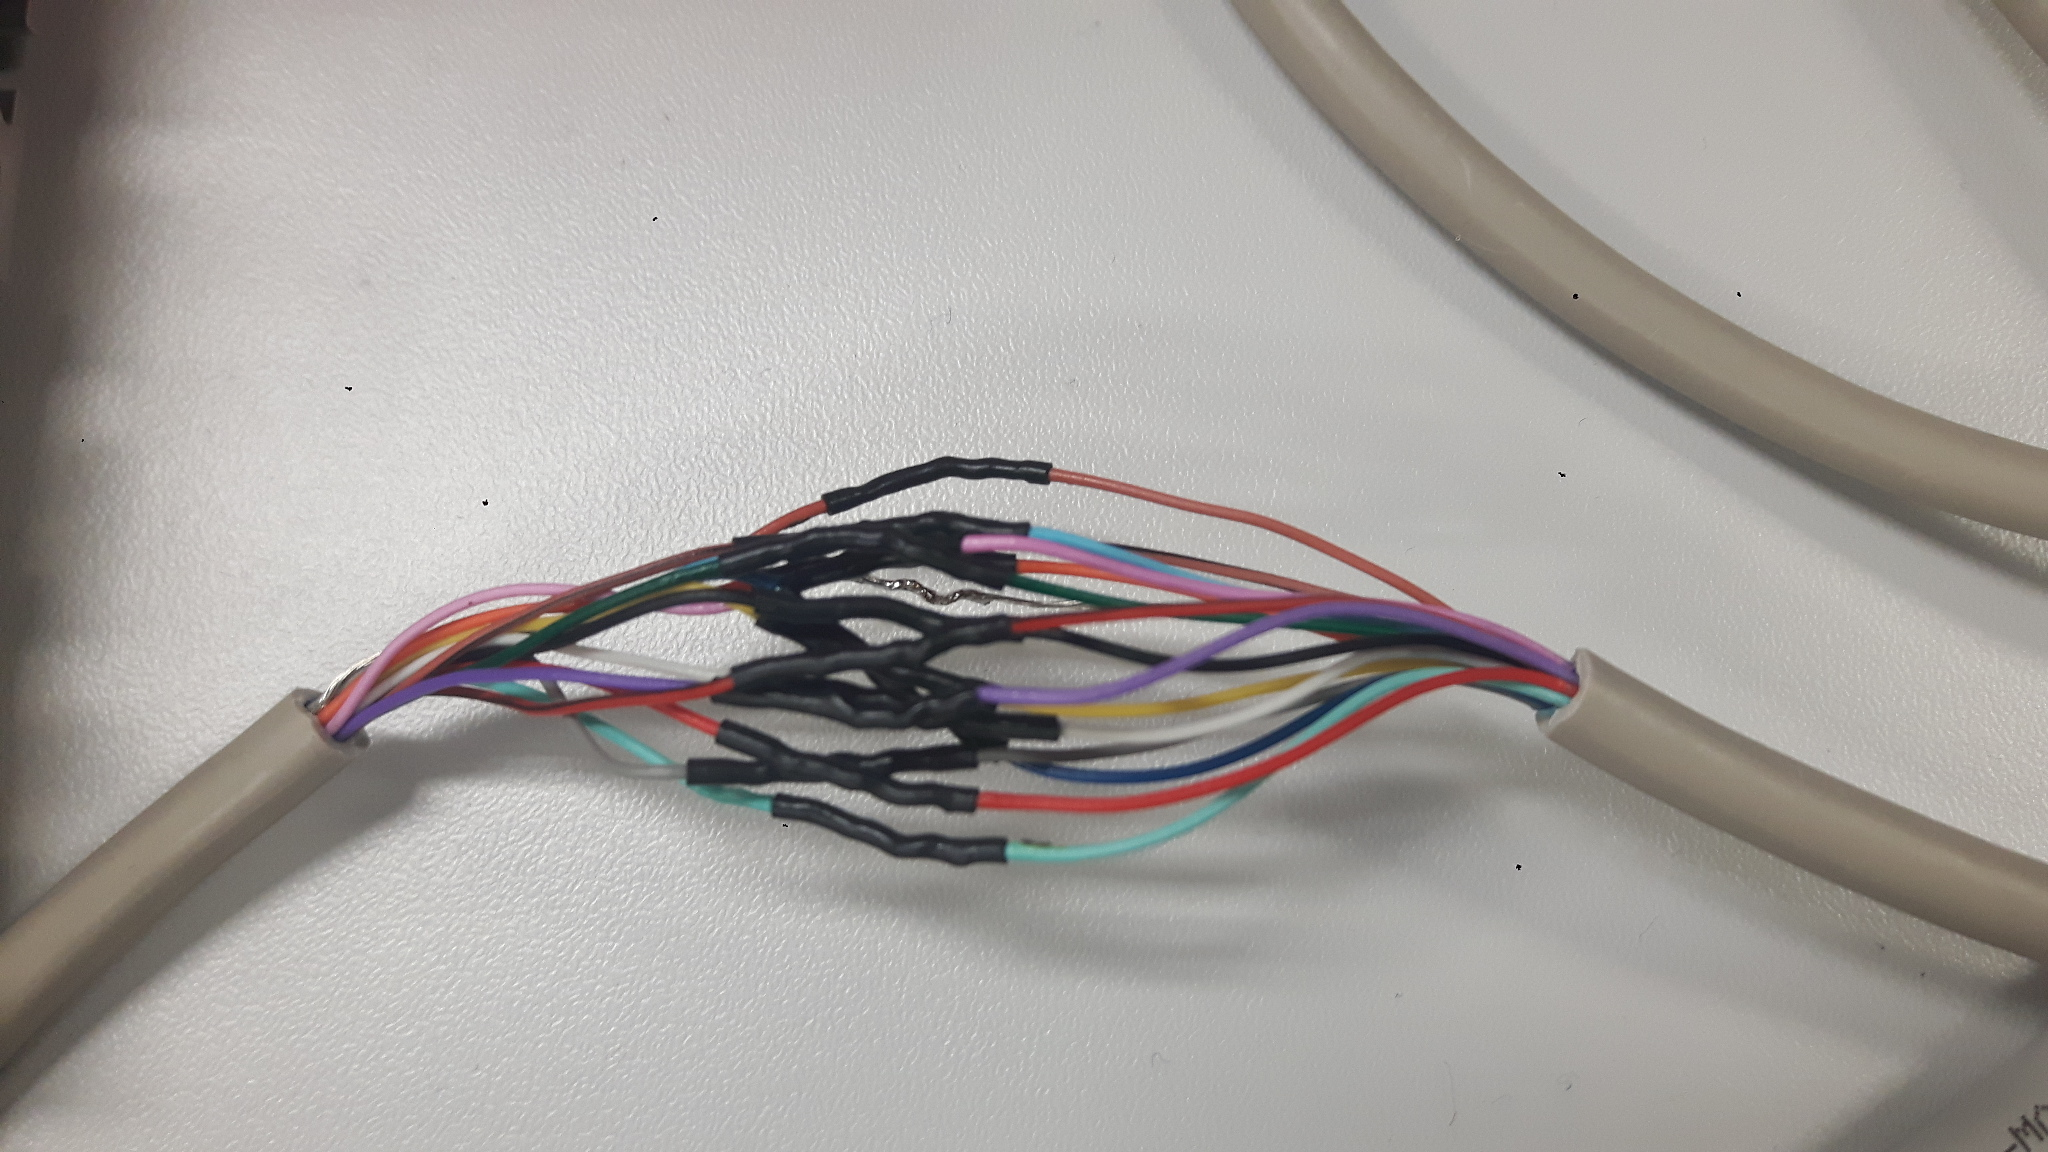
\includegraphics[scale=0.10]{kabel.jpg}
	  \caption{DB15 Kabel}
	\label{kabel}
\end{figure}

Dank des Y-Schalters kann diese Arbeit daher die vom Buskoppler kommenden Signale und des Prozesses lesen. Ich habe mich für einen Raspberry Pi 3 entschieden, bei dem es sich um einen Einplatinencomputer handelt, der das Raspbian-Betriebssystem verwendet, das ein Derivat von Debian ist. Dieser kleine Computer kann über einen HDMI-Anschluss an einen Bildschirm angeschlossen werden und wird einfach mit 5 V betrieben. Der Raspberry Pi ist ein kostengünstiger Computer mit rund 40 Euro, einfach zu bedienen und weit verbreitet, sodass Sie leicht Tutorials oder darauf angepasste Hardware / Software finden können. 

\begin{figure}[ht!]
	\centering
	  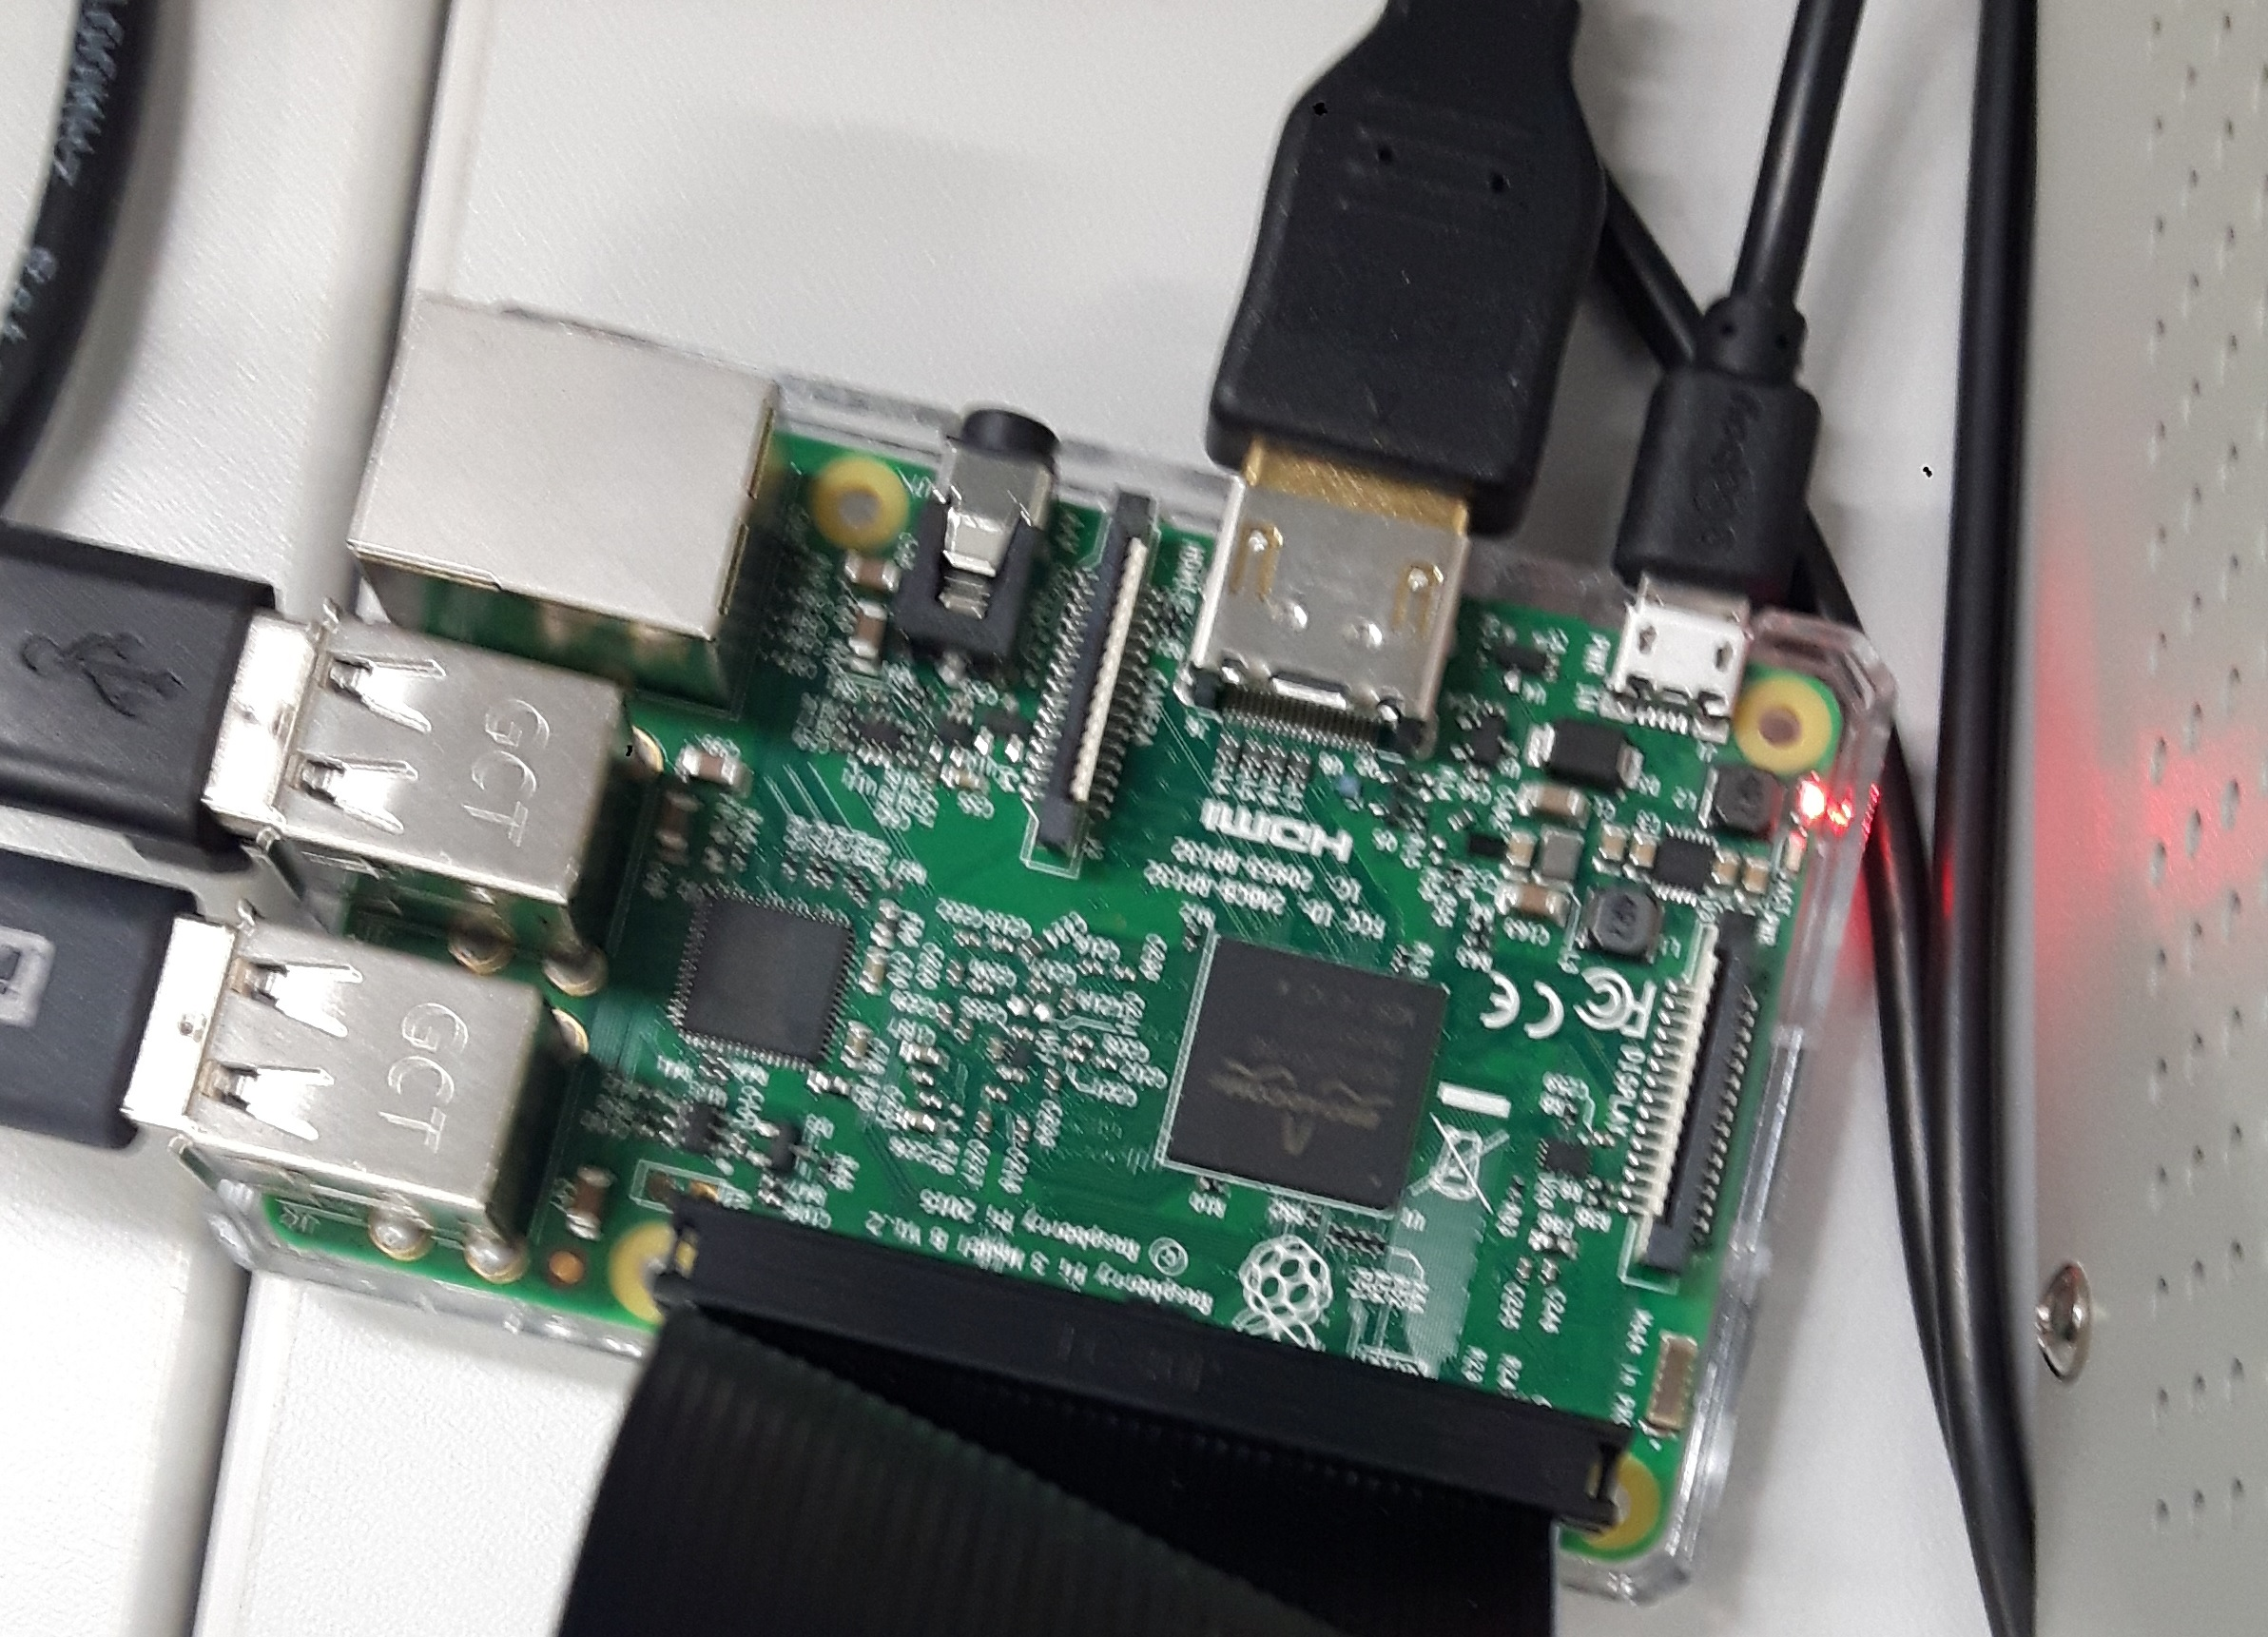
\includegraphics[scale=0.15]{raspberry.jpg}
	  \caption{Raspberry Pi 3}
\end{figure}

Es verfügt über vier USB-Anschlüsse, an die Sie eine Speichererweiterung anschließen können, z. B. eine externe Festplatte / SSD. Dank dieser 40 GPIO-Anschlüsse (General Purpose Input / Output) kann der Raspberry eine kontinuierliche Spannung von 3,3 V und 5 V liefern und digitale Daten lesen oder senden. Da nur digitale Signale gelesen werden, muss ein Analog-Digital-Wandler verwendet werden. Ich habe mich für den MCP3008 entschieden, einen Wandler, der regelmäßig für diese Art von Hardware verwendet wird, nämlich die Raspberry. Dieser Wandler verfügt über acht analoge Eingangskanäle und einen digitalen Ausgangskanal. 

\begin{figure}[ht!]
	\centering
	  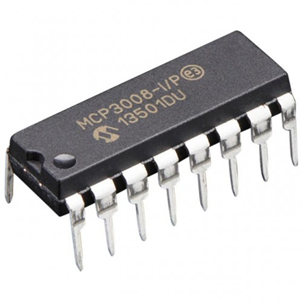
\includegraphics[scale=0.5]{converter.png}
	  \caption[AD Converter MCP3008]{AD Converter MCP3008\footnotemark}
\end{figure}

\footnotetext{https://www.overleaf.com/learn/latex/Footnotes}

Der Konverter kann jedoch nur analoge Signale lesen, deren Spannungswert weniger als 3 V beträgt, wenn er mit der 3,3-V-Stromversorgung der Raspberry versorgt wird. Alle Analogwerte größer als 3 V am Eingang werden daher standardmäßig auf den Wert 3 V gesetzt. Es besteht daher die Notwendigkeit, eine Schaltung zu erzeugen, um die zum Wandler gehende Spannung zu verringern. Diese Schaltung dient auch als Schutz für die Raspberry, da sie keine Spannungen über 5 V unterstützt. 

\begin{figure}[ht!]
	\centering
	  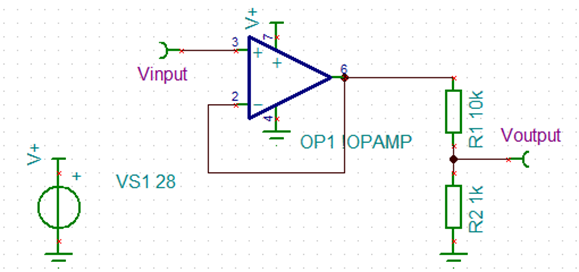
\includegraphics[scale=0.5]{montage.png}
	  \caption{Spannung Reduktion Montage}
\end{figure}

Die hergestellte elektronische Baugruppe besteht aus einem Operationsverstärker, der dazu dient, die Baugruppe vom Y-Schalter zu isolieren, und einer Spannungsteilerbrücke, die die Spannung um ungefähr 10 verringert. 

\begin{align}
V_{output} = \frac{R_{1}}{R_{1} + R_{2}} \cdot V_{input} \\
V_{output} = 0,1 \cdot V_{input} \nonumber
\label{eq:}
\end{align}

Der verwendete Operationsverstärker ist ein LM324N, der asymmetrisch mit 28 V versorgt wird. Die komplette Baugruppe mit der elektrischen Baugruppe und der Raspberry ist in der Abbildung \ref{montage} dargestellt. 

\begin{figure}[ht!]
	\centering
	  \includegraphics[angle=-90,origin=c,scale=0.04]{ganze_montage_mit_raspberry.jpg}
	  \caption{Ganze Montage}
	\label{montage}
\end{figure}

\subsection{Signalanalyse}

Das System kommuniziert mit vier Signalen mit dem Prozess und umgekehrt kommuniziert der Prozess zu vier Signalen mit dem System. Das System weist den Prozess an, die Schranke abzusenken, das Laufband nach rechts oder links zu schalten und das Licht ein- oder auszuschalten. Der Prozess hingegen informiert das System über den Zustand des induktiven Sensors, Lichtschranke, Schalter und Taster. Alle diese Signale werden von SAAD abgegriffen und die verschiedenen Signalformen untersucht. Die Signale wurden mit einer Frequenzabtastung von 33 Hz abgegriffen.  
Das Schranke-Signal zeigt an, wann der Befehl zum Absenken gegeben wird. Die Schranke senkt sich nur, wenn der in den Prozess eingesetzte Topf der silberen Topf ist. Die Abbildung \ref{schranke} zeigt die beiden Möglichkeiten des Signals. 

\begin{figure}[ht!]
	\centering
	  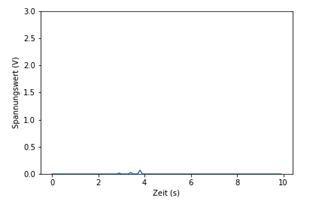
\includegraphics[scale=0.75]{schranke_black.png}
	  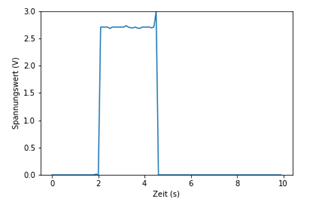
\includegraphics[scale=0.75]{schranke.png}
	  \caption{Schranke Signale für silbern Topf (rechts) und schwarz Topf (links)}
	  \label{schranke}
\end{figure}

Das Material des Topfes wird vom induktiven Sensor erfasst, der die Informationen an das System sendet, das die Entscheidung trifft, ob die Schranke abgesenkt werden soll oder nicht. Das Signal für den induktiven Sensor wird durch die Abbildung für die beiden Fälle silbern und schwarz Topf dargestellt. 

\begin{figure}[ht!]
	\centering
	  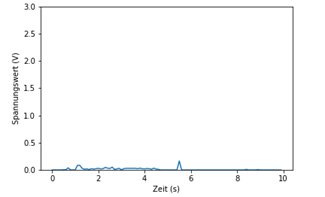
\includegraphics[scale=0.75]{induktiv_sensor_black.png}
	  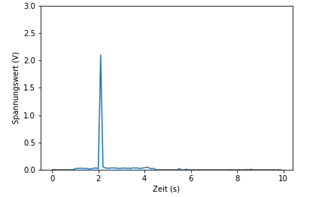
\includegraphics[scale=0.75]{induktiv_sensor.png}
	  \caption{Induktive Sensor Signale für silbern Topf (rechts) und schwarz Topf (links)}
	  \label{induktiv_sensor}
\end{figure}

Der Schalter zeigt an, ob der Prozess am System eingeschaltet ist oder nicht. Die Messung des Signals beim Einspeisen des Prozesses durch Drehen des Schalters ist in der Abbildung \ref{schalter} dargestellt. In derselben Abbildung ist das Signal für das Licht dargestellt. Wenn der Prozess eingeschaltet ist, blinkt das Licht und wenn der Prozess verwendet wird, bleibt das Licht an. 

\begin{figure}[ht!]
	\centering
	  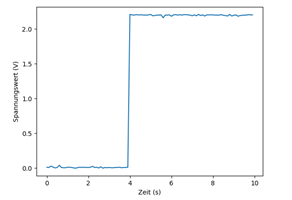
\includegraphics[scale=0.75]{schalter.png}
	  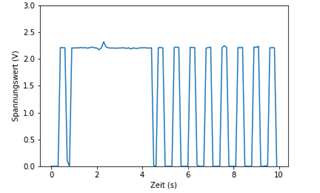
\includegraphics[scale=0.75]{licht.png}
	  \caption{Schalter Signal (links) und Licht Signal (rechts)}
	  \label{schalter}
\end{figure}

In der Abbildung \ref{lichtschranke} links sind die Signale für die Lichtschranke dargestellt, die erkennen, wann ein Objekt durch sie hindurchgeht, und so das Laufband sich nach rechts bewegt. Die Abbildung rechts zeigt das Taster Signal. Wenn der Taster gedrückt wird, beginnt das Laufband links zu bewegen. 

\begin{figure}[ht!]
	\centering
	  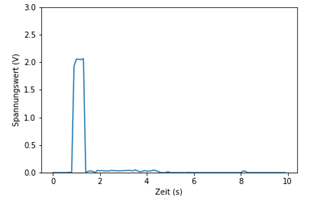
\includegraphics[scale=0.75]{lichtschranke.png}
	  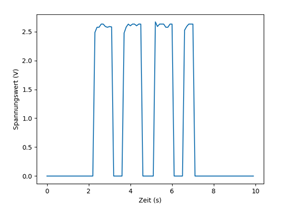
\includegraphics[scale=0.75]{taster.png}
	  \caption{Lichtschranke Signal (links) und Taster Signal (rechts)}
	  \label{lichtschranke}
\end{figure}

In der Abbildung \ref{laufband} zeigen die Signale an, wann sich das Laufband im konventionellen Betrieb befindet, d.h. nach rechts bewegt und wann das Laufband nach dem Drücken des Tasters nach links bewegt. 

\begin{figure}[ht!]
	\centering
	  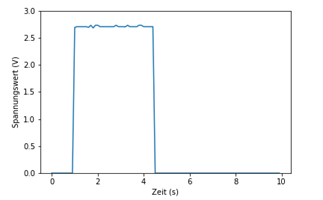
\includegraphics[scale=0.75]{laufband.png}
	  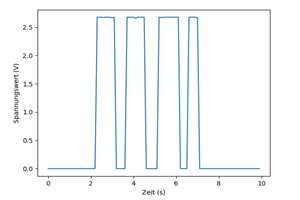
\includegraphics[scale=0.75]{laufbandlinks.png}
	  \caption{Laufband Signal (links) und Laufband nach links Signal (rechts)}
	  \label{laufband}
\end{figure}

Nachdem diese Arbeit alle Signale wiederhergestellt hatte, führt diese Arbeit eine statistische Analyse der Signale für jeden Sensor durch, die in einer Datenbank zentral gespeichert wurden. Diese umfasste 60 Läufe mit einem silbernen Topf, 60 Läufe mit einem schwarzen Topf, zehn Läufe mit dem verwendeten Stop-Button-Notfall und drei Läufe bei Verwendung des Tasters.
Eine Zusammenfassung der für jeden Sensor erhaltenen Werte ist in der Tabelle \ref{stat} gezeigt. 

 \begin{table}[ht!]
    \begin{tabular}{|p{1.2cm}|*{9}{@{\hskip.2mm}c@{\hskip.2mm}|}}
    \hline
No Scaler &	Schranke &	Laufband &	Taster &	Band Links &	Ind. Sensor &	Licht &	Schalter &	Lichtschranke \\ \hline
count &		60300 &		60300	 &	60300 &		60300 &		60300 &		60300	 &	60300 &		60300 \\ \hline
mean &		0,356 &		0,996 &		0,01 &		0,010 &		0,022 &		1,532 &		2,044 &		0,096 \\ \hline
std &		0,916 &		1,308 &		0,138	 &	0,140 &		0,171 &		1,016 &		0,543 &		0,419 \\ \hline
min	 &	0 &		0	 &	0	 &	0 &		0 &		0 &		0 &		0 \\ \hline
25\% &		0 &		0 &		0 &		0 &		0 &		0 &		2,172 &		0 \\ \hline
50\% &		0 &		0 &		0	 &	0	 &	0	 &	2,204 &		2,198 &		0 \\ \hline
75\% &		0 &		2,720	 &	0	 &	0 &		0,016 &		2,211	 &	2,204 &		0,0161 \\ \hline
max &		3,116	 &	3,100	 &	2 &		2 &		2,224 &		2,427	 &	2,414 &		2,295 \\ \hline


    \end{tabular}
    \caption{Statistische Werte für jeden Sensoren}
    \label{stat}          
\end{table}

Gemäß dieser Tabelle können wir abnormale Maximalwerte sehen, da der Prozess mit 24 V versorgt wird. Dann sollten wir keine Werte über 2,4 V erhalten, da diese Werte nach Division der Spannung durch 10 erhalten werden. Diese Maximalwerte können auf mögliche Spannungsspitzen im Prozess oder auf elektronisches Rauschen des Y-Schalters oder der Spannungsreduzierungsschaltung zurückzuführen sein. Da diese Spannungsspitzen selten sind und einen schwachen Einfluss auf die Form des Signals haben, habe ich daher keine Initiative ergriffen, um dieses Rauschen zu reduzieren. 

Diese Arbeit hat auch die Kovarianzmatrix der Sensorsignale berechnet. Diese Matrix wird in Tabelle 2 dargestellt. Dank dieser Matrix können wir die Varianz für einen bestimmten Sensor, aber auch die Kovarianz zwischen zwei Sensoren für die ausgewählten Daten ableiten. Wir stellen fest, dass die Varianz für das Laufband am größten ist, was normal ist, da das Laufband bei Verwendung des Prozesses notwendigerweise in Betrieb ist, da das Laufband in Betrieb geht und so lange in Betrieb bleibt, sobald ein Objekt über die Lichtschranke erkannt wird bis der Topf sortiert wird. Wenn man den Taster drückt, ist auch das Laufband in Betrieb. Umgekehrt ist die Varianz für den induktiven Sensor gering, da er nur dazu dient, die Information an den Buskoppler und die SPS zu senden, dass die Schranke abgesenkt werden muss. 

 \begin{table}[ht!]
    \begin{tabular}{|p{1.6cm}|*{9}{@{\hskip.2mm}c@{\hskip.2mm}|}}
    \hline
No Scaler &	Schranke &	Laufband &	Taster &	Band Links &	Ind. Sensor &	Licht &	Schalter &	Lichtschranke \\ \hline
Schranke runter &		0,842 &		0,592 &		-0,003 &		-0,004 &		0,03 &		0,229 &		0,009 &		-0,025 \\ \hline
Laufband &		0,592 &		1,71 &		0,010 &		0,011 &		0,033 &		0,658 &		0,023 &		0,145 \\ \hline
Taster &		-0,003 &		0,010 &		0,019 &		0,019 &		0 &		-0,004 &		0 &		-0,001 \\ \hline
Band nach links &		-0,0035 &		0,0105 &		0,0190 &		0,0196 &		-0,0002 &		-0,0041 &		0 &		-0,001 \\ \hline
Induktiv Sensor &		0,03 &		0,033 &		0 &		0 &		0,029 &		0,013 &		0,002 &		0 \\ \hline
Licht an &		0,229 &		0,658 &		-0,004 &		-0,004 &		0,013 &		1,032 &		-0,043 &		0,059 \\ \hline
Schalter &		0,009 &		0,023 &		0 &		0 &		0,002 &		-0,043 &		0,295 &		0,011 \\ \hline
Licht- schranke &		-0,025 &		0,145 &		-0,001	 &	-0,001 &		0 &		0,059 &		0,011 &		0,175 \\ \hline

    \end{tabular}
    \caption{Kovarianzmatrix}
    \label{kov}          
\end{table}

Aus der Korrelationsmatrix können wir daher die Beziehungen zwischen jedem Sensor überprüfen und die Abhängigkeit der Sensoren miteinander erkennen. Aus Tabelle 3 können wir daher ersehen, dass das Laufband dasjenige ist, das die größte Korrelation mit den anderen Sensoren aufweist. Dieses Ergebnis ist ziemlich logisch, da das Laufband bereits in Betrieb ist, wenn ein anderes Element als das Laufband verwendet wird. Wir beobachten auch, dass der induktive Sensor die größte Korrelation mit der Schranke aufweist. Auch dieses Ergebnis ist normal, denn wenn der induktive Sensor den Silberschaufel erkennt, muss die Schranke schließen. 

 \begin{table}[ht!]
    \begin{tabular}{|p{1.6cm}|*{9}{@{\hskip.2mm}c@{\hskip.2mm}|}}
    \hline
No Scaler &	Schranke &	Laufband &	Taster &	Band Links &	Ind. Sensor &	Licht &	Schalter &	Lichtschranke \\ \hline
Schranke runter &		1,000 &		0,494 &		-0,027 &		-0,027 &		0,189 &		0,246 &		0,018 &		-0,064 \\ \hline
Laufband &		0,494 &		1,000 &		0,057 &		0,057 &		0,149 &		0,496 &		0,033 &		0,265 \\ \hline
Taster &		-0,027 &		0,057 &		1,000 &		0,983 &		-0,008 &		-0,026 &		-0,006 &		-0,015 \\ \hline
Band nach links &		-0,027 &		0,057 &		0,983 &		1,000 &		-0,009 &		-0,029 &		-0,006 &		-0,015 \\ \hline
Induktiv Sensor &		0,189 &		0,149 &		-0,008 &		-0,009 &		1,000 &		0,076 &		0,025 &		0,001 \\ \hline
Licht an &		0,246 &		0,496 &		-0,026 &		-0,029 &		0,076 &		1,000 &		-0,079 &		0,139 \\ \hline
Schalter &		0,018 &		0,033 &		-0,006 &		-0,006 &		0,025 &		-0,079 &		1,000 &		0,050 \\ \hline
Licht- schranke &		-0,064 &		0,265 &		-0,015 &		-0,015 &		0,001 &		0,139 &		0,050 &		1,000 \\ \hline

    \end{tabular}
    \caption{Korrelationsmatrix}
    \label{korr}          
\end{table}

Anschließend dienen diese Tabellen als Referenz, da diese Arbeit, wie wir sehen werden, verschiedenen Scalers auf die Daten anwenden werden, um ihren Einfluss auf die Anomalieerkennungsmethoden zu beobachten und sie zu klassifizieren, um zu wissen, welcher Scaler das beste Ergebnis liefert. Diese Tabellen werden daher verwendet, um zu beobachten, wie die Scalers die Werte der Signale ändern. 

\clearpage
%%%%%%%%%%%%%%%%%%%%%%%%%%%%%%%%%
 \newpage  % neuer Abschnitt auf neue Seite, kann auch entfallen
%%%%%%%%%%%%%%%%%%%%%%%%%%%%%%%%%
\section{Analyse}
\subsection{Angriff}

Bevor die verschiedenen bereits vorhandenen Angriffe und ihre Auswirkungen auf den Prozess beschrieben werden, wird zunächst das normale Verhalten des Prozesses definiert, d.h. die Signale, die die Methoden lernen müssen, um Anomalien zu erkennen.
Der Prozess umfasst vier normale Verhaltensweisen. Die ersten beiden Verhaltensweisen treten bei der Einführung eines silbernen oder schwarzen Topfes auf. 

Die Abbildung \ref{regroup} repräsentiert die Form der Signale für jeden Sensor für ein Verhalten mit einem silbernen und schwarzen Topf. Wenn ein silberner Topf in den Prozess eingesetzt wird, erkennt die Lichtschranke ihre Anwesenheit und aktiviert das Laufband, welches sich dann in Fahrtrichtung rechts bewegt. Gleichzeitig bleibt das Licht an. Wenn der Topf vor dem induktiven Sensor vorbeifährt, erkennt er das Material, und die Schranke wird abgesenkt. Nach einigen Sekunden, wenn der Silberne Topf die Rampe heruntergefahren ist, steigt die Schranke wider an, das Laufband stoppt und das Licht blinkt erneut. Das Verhalten ist für den schwarzen Topf das gleiche, mit dem Unterschied, dass es vom induktiven Sensor nicht erkannt wird und die Schranke daher nicht herunterfährt. 

\begin{figure}[ht!]
	\centering
	  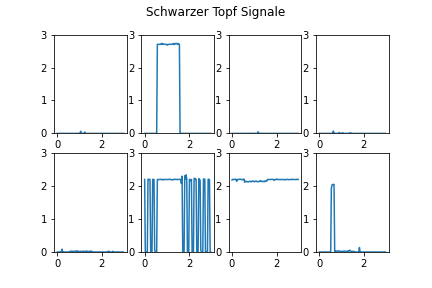
\includegraphics[scale=0.5]{black_signal.png}
	  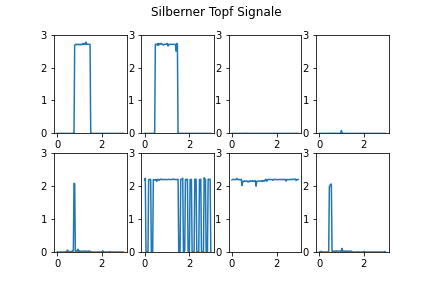
\includegraphics[scale=0.5]{silver_signal.png}
	  \caption{Normales Verhalten mit silbernen (rechts) und schwarzen Topf (links)}
	 \label{regroup}
\end{figure}

Ein weiteres normales Verhalten ist, wenn man den Taster drückt und sich das Laufband nach links bewegt. Es erscheint also drei Signale, eines zeigt an, dass der Taster gedrückt ist, ein zweites zeigt an, dass sich das Laufband bewegt, und ein drittes zeigt an, dass sich das Laufband nach links bewegt. Die Signale für dieses Verhalten sind in der Abbildung \ref{taster_verhalten} dargestellt. 

\begin{figure}[ht!]
	\centering
	  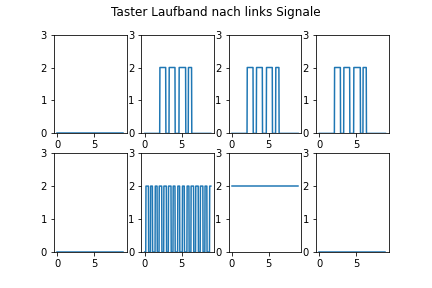
\includegraphics[scale=0.5]{taster_regroup.png}
	  \caption{Normalen Verhalten mit Taster}
	\label{taster_verhalten}
\end{figure}

Das letzte normale Verhalten ist das des Not-Aus-Tasters. Beim Drücken wird die Stromzufuhr zum Prozess unterbrochen und daher nicht mehr mit Strom versorgt, der das Laufband stoppt und das Licht ausschaltet. Dieses Verhalten ist in Abbildung \ref{notaustaster} dargestellt. \\

\begin{figure}[ht!]
	\centering
	  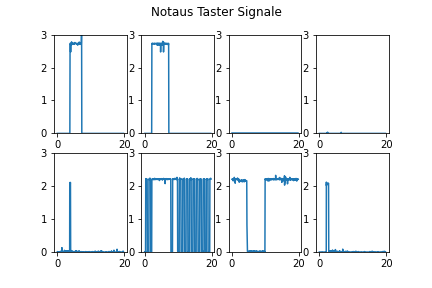
\includegraphics[scale=0.5]{notaustaster.png}
	  \caption{Normalen Verhalten mit Not-aus Taster}
	\label{notaustaster}
\end{figure}

Es gibt zwei Arten von Angriffen, die sich auf ein industrielles System auswirken können. Die erste Art von Angriff ändert das normale Verhalten des Systems, um die Produktionslinie zu verlangsamen oder Geräte zu zerstören. Für diese Art von Angriffen sind zwei Angriffe vorhanden: PLCinject und Profinet-Replay. Per PLCinject wird Schadcode auf die primäre SPS eingespielt. Durch einen Profinet-Replay-Angriff auf den Profinet-Buskoppler werden die Anweisungen der SPS ignoriert und das Prozessverhalten geändert, zum Beispiel, läuft das Laufband  in die falsche Richtung. Das Funktionsprinzip wird durch die Abbildung \ref{ganze_systeme} dargestellt. Diese Art von Angriff muss von SAAD erkannt werden. Die zweite Angriffsart ändert in keiner Weise das ursprüngliche Verhalten des Prozesses und sollte daher von SAAD nicht erkannt werden. \\

\begin{figure}[ht!]
	\centering
	  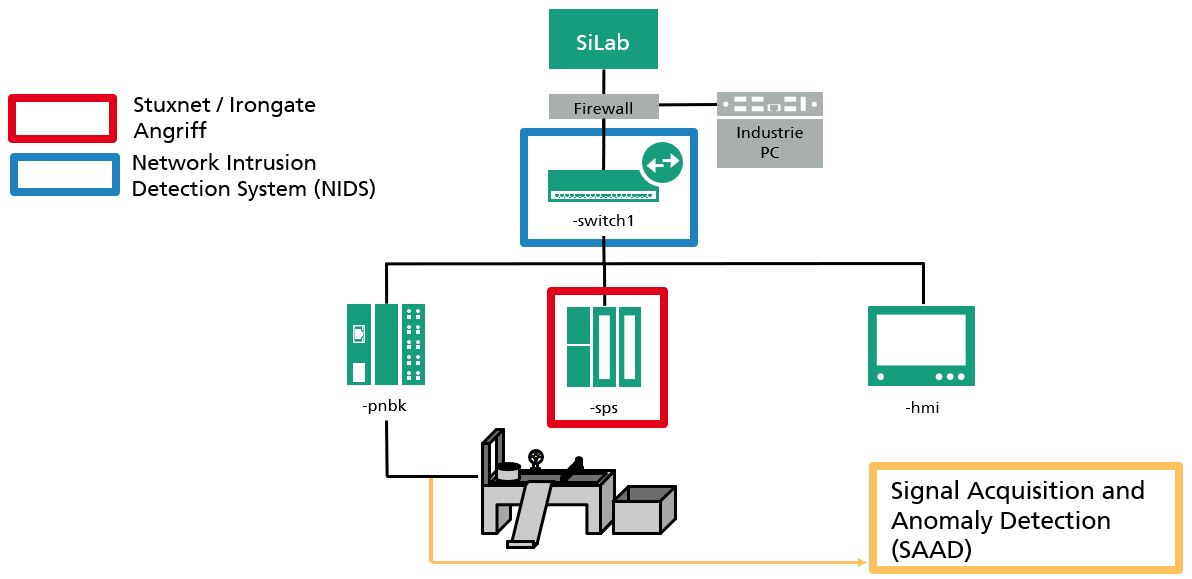
\includegraphics[scale=0.5]{ganze_systeme.jpg}
	  \caption{Industrielle System Beispiel}
	\label{ganze_systeme}
\end{figure}


In unserem Fall haben wir drei Angriffe, die das normale Verhalten des Prozesses ändern können, und einen Angriff, der keine Konsequenzen für den Prozess hat. Alle diese Angriffe werden über den Switch mithilfe eines mit Software ausgestatteten Computers in das System eingespeist, mit dessen Hilfe die Kommunikation in einem industriellen System wie Wireshark analysiert werden kann.

Einer der Angriffe, die das normale Verhalten des Prozesses beeinflussen können, ist der Rename Angriff. Der Zweck dieses Angriffs besteht darin, ein Element des Systems umzubenennen. Auf diese Weise können die anderen Elemente des Systems es nicht mehr finden und mit ihm kommunizieren. In unserem Fall wurde der Buskoppler umbenannt. Folglich kann die SPS, die dessen "neuen" Namen nicht mehr kennt, nicht mehr mit dem Buskoppler kommunizieren. Dies hat zur Folge, dass verhindert wird, dass Kommunikationen vom Buskoppler und damit von der SPS zum Prozess gelangen. Es ist in der Tat für jeden leicht, diese Art von Angriff auf industrielle Systeme durchzuführen, da das Kommunikationsprotokoll keine Sicherheitsmechanismen umsetzt. Die Signale des Angriffes wird durch die Abbildung \ref{rename_angriff} dargestellt.

\begin{figure}[ht!]
	\centering
	  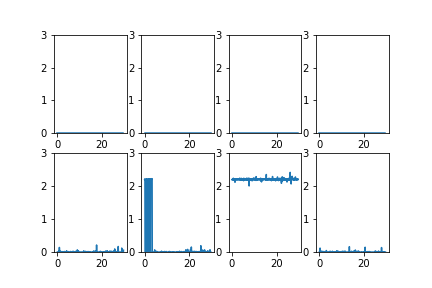
\includegraphics[scale=0.75]{rename_angriff.png}
	  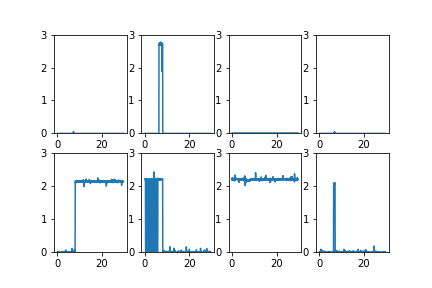
\includegraphics[scale=0.75]{rename_angriff_process_on.png}
	  \caption{Rename Angriff Signale, Prozess in Betrieb (rechts) und Prozess nicht in Betrieb (links)}
	\label{rename_angriff}
\end{figure}

Ein weiterer Angriff, der das System verändern kann, ist der Replay Angriff. Dieser Angriff aktiviert das Laufband, jedoch bewegt sich das Laufband in die falsche Richtung, nämlich nach links. Wenn der Prozess in Betrieb ist, stoppt der Prozess und bewegt das Laufband links. Diese Verhaltensweisen sind in der Abbildung \ref{replay} dargestellt. 

\begin{figure}[ht!]
	\centering
	  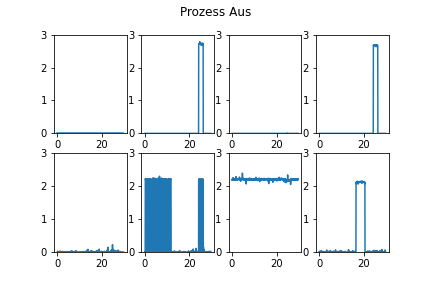
\includegraphics[scale=0.5]{replay_angriff.png}
	  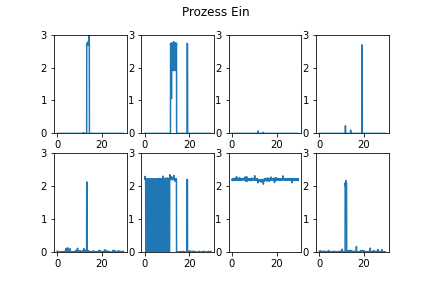
\includegraphics[scale=0.5]{replay_angriff_process_on.png}
	  \caption{Replay Angriff Signale, Prozess in Betrieb (rechts) und Prozess nicht in Betrieb (links)}
	\label{replay}
\end{figure}

Der letzte Angriff, der das Verhalten des Systems ändert, ist an sich kein wirklicher Angriff, da er nicht durch Injizieren eines Computerwurms oder durch Ändern eines Teils des Systems ausgeführt wurde. Es wurde Simulated Angriff genannt. Ein Lauf wurde mit einem silbernen Topf und dann einen mit dem schwarzen Topf aufgenommen. Dann wurden die Schranke Signale zwischen den beiden Läufen ausgetauscht, das heißt, während dieser Fehlfunktion beim Einsetzen des Silber-Topfes wird dieser von der Lichtschranke erkannt und das Laufband beginnt sich nach rechts zu bewegen. Das Material des silberne Topfes wird vom induktiven Sensor gut erkannt, aber die Schranke sinkt nicht ab. Bei einem Lauf mit einem schwarzen Topf finden wir das klassische Verhalten des Prozesses mit dem Unterschied, dass die Schranke sinkt. Diese Verhaltensweisen werden durch die Abbildung \ref{fake} dargestellt. Diese Art von falschem Angriff kann mit Shadcode verglichen werden, bei dem wir den Vorgang umkehren. Ein Beispiel für die Verwendung eines Angriffs könnte der Angriff eines industriellen Lebensmittelsystems sein, bei dem festgestellt wird, ob ein Lebensmittel, beispielsweise ein Gemüse, aufgrund seiner Farbe verfault ist oder nicht. Faule Lebensmittel würden nicht länger von den Zutaten ausgeschlossen, und umgekehrt würden gute Lebensmittel ausgeschlossen. Wir können uns diese Art von Angriff in jeder Art von industriellem System, das Objekte nach ihren Farben oder ihrem Material sortiert, genauso gut vorstellen wie in einem metallurgischen industriellen System. 

\begin{figure}[ht!]
	\centering
	  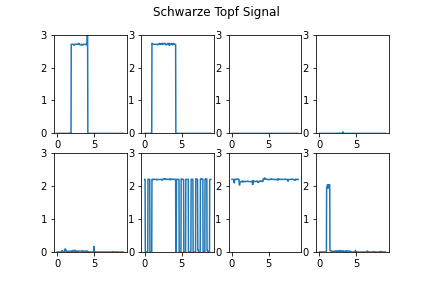
\includegraphics[scale=0.5]{fake_angriff_black.png}
	  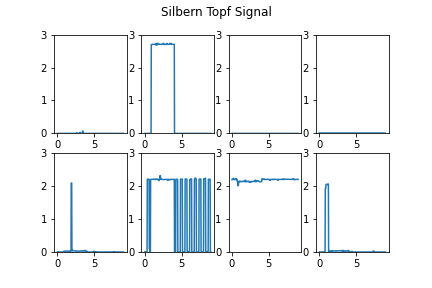
\includegraphics[scale=0.5]{fake_angriff_silver.png}
	  \caption{Fake Angriff Signale für schwarz Topf (links) und silbern Topf (rechts)}
	\label{fake}
\end{figure}

Um SAAD weiter zu testen, hat diese Arbeit einen Angriff in das System injiziert, der das Verhalten des Prozesses nicht ändert, aber dennoch Konsequenzen für das System hat. Dieser Angriff ist der Safety Angriff. Damit soll verhindert werden, dass die Stromversorgung des Systems unterbrochen wird, wenn der Not-Aus-Taster gedrückt wird. Daher stoppt der Prozess nicht mehr, wenn die Not-Aus-Taste gedrückt wird, und läuft weiter, wenn ein Topf in den Prozess eingefügt wurde. Diese Verhaltensweisen werden durch die Abbildung \ref{sis_angriff_process} dargestellt.

\begin{figure}[ht!]
	\centering
	  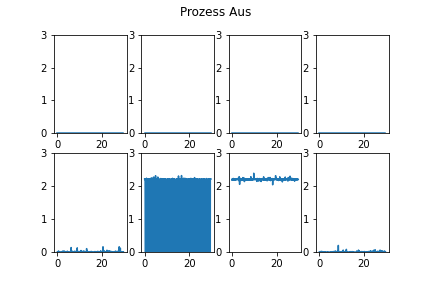
\includegraphics[scale=0.5]{sis_angriff.png}
	  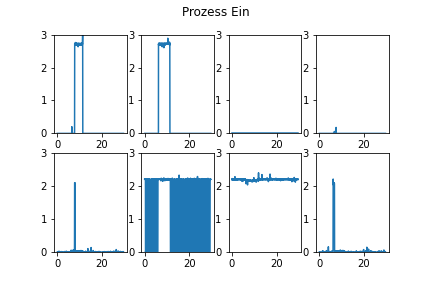
\includegraphics[scale=0.5]{sis_angriff_process_on.png}
	  \caption{Safety Angriff Signale, Prozess in Betrieb (rechts) und Prozess nicht in Betrieb (links)}
	\label{sis_angriff_process}
\end{figure}

\subsection{Implementierung}
 
Der Code besteht aus zwei Hauptteilen, einem Datenerfassungsteil und einem Anomalieerkennungsteil. In beiden Fällen wird Python als Programmiersprache verwendet. Für den Erfassungsteil werden Busio, Digitalio, Board und Bibliotheken verwendet. Es wird verwendet, um den AD-Wandler zu initialisieren und jedem verwendeten Kanal eine Variable zuzuweisen. Die Bibliotheken numpy\footnotemark{} und matplotlib\footnotemark{} werden verwendet, um die Daten in Form von Bildern und Binärdateien zu speichern, die später verwendet werden können.

\footnotetext{https://numpy.org/}
\footnotetext{https://matplotlib.org/stable/index.html}

Für den Teil zur Erkennung von Anomalien werden die Bibliotheken von Pytorch\footnotemark{} und sklearn [8] zur Implementierung von Methoden zur Erkennung einer Anomalie verwendet. Die Panda-Bibliothek dient zur statistischen Analyse von Daten. Die Bibliotheken numpy und matplotlib werden verwendet, um die Daten in Form von Binärdateien zu lesen und die verschiedenen Ergebnisse anzuzeigen.

\footnotetext{https://pytorch.org/}

Für die CNN- und Autoencoder-Methoden hat diese Arbeit den Einfluss der No Scaler-, BooleanScaler-Scaler mit einem Schwellenwert von 1 verglichen, da dies den Durchschnittswert zwischen dem Maximal- und Minimalwert für MinMaxScaler und StandardScaler darstellt. In Teil 6.2 wird erklären was ein Scaler ist. Für das CNN-Verfahren werden Fenster unterschiedlicher Länge angewendet, die von 5 Datenpunkten, was einer Sechstelsekunde entspricht, bis zu 66 Datenpunkten, die ein Zwei-Sekunden-Fenster sind, reichen.
Für die Autoencoder-Methode wurde ein einzelnes Fenster mit der Größe $8*40 = 320$ verwendet. 

Für das SVM hat diese Arbeit den Parameter "nu" geändert, der eine Obergrenze für den Anteil der Trainingsfehler und eine Untergrenze für den Anteil der Unterstützungsvektoren darstellt. Durch Verringern dieses Parameters erhalten wir bessere Ergebnisse für die Erkennung vom Normalverhalten, aber schlechte Ergebnisse für die Erkennung von Anomalien. Durch Erhöhen dieses Parameters können wir bessere skalierungsabhängige Ergebnisse erzielen.

Für LOF muss mit der Anzahl der Nachbarn experimentiert werden, um die Dichteabweichung einer Probe zu berechnen. Durch Ändern dieses Parameters werden je nach Scaler unterschiedliche Verhaltensweisen beobachtet, was bei einigen Scalern zu guten Ergebnissen bei einem niedrigen Wert der Anzahl der Nachbarn führen kann, während bei anderen Scaler eine große Anzahl von Nachbarn erforderlich ist, um eine korrekte Anomalieerkennung zu erzielen.

Für DBSCAN experimentiert diese Arbeit mit dem Parameter, der den maximalen Abstand zwischen zwei Samples darstellen, damit sie in demselben Sample berücksichtigt werden, und mit dem Parameter, welches die mindeste Anzahl von Samples in einer Nachbarschaft darstellt, damit dies als Kernpunkt betrachtet wird. Diese beiden Parameter wurden so gewählt, dass DBSCAN ein einzelnes Cluster erkennt, wobei der eine das normale Verhalten des Prozesses neu gruppiert und alle Ausreißer die Punkte sind, die eine Anomalie erkennen.

%%%%%%%%%%%%%%%%%%%%%%%%%%%%%%%%%
 \newpage  % neuer Abschnitt auf neue Seite, kann auch entfallen
%%%%%%%%%%%%%%%%%%%%%%%%%%%%%%%%%
\section{Evaluation}

In diesem Teil wird erläutert, welche Datensätze verwendet werden und welche Scaler auf sie angewendet wurden. Es wird auch die Auswirkung von Scalern auf einen Datensatz gezeigt. Es wird auch erklärt, wie die Modelle trainiert wurden und mit welchen Methoden die Modelle bewertet wurden. 

\subsection{Dataset}

Mithilfe des Raspberry Pi wurden 133 Läufe mit normalem Verhalten und zwei Läufe für jeden Angriff abgegriffen. Aus dem Datensatz mit den 133 Läufen mit normalem Verhalten wurden zwei Datensätze erstellt: ein Trainingsdatensatz und ein Testdatensatz. Der Trainingsdatensatz wird zum Trainieren von Modellen unter Verwendung neuronaler Netze verwendet.

Der Testdatensatz wird verwendet, um die Leistung von Modellen zu überprüfen, wenn nur normales Verhalten erkannt werden muss. Wie unten gezeigt, erfolgt die Optimierung der Anomalieerkennung zum Nachteil der Erkennung normaler Verhaltensweisen. In einem industriellen System erfolgt die Erkennung jedoch größtenteils in Echtzeit, es erfolgt kein Angriff, und daher darf SAAD keine Anomalie erkennen. Wenn das System auch ohne Angriffe ständig nur Anomalien erkennt, ist solch ein System praktisch nicht brauchbar und einsetzbar.

Zur Erkennung von Anomalien enthält jeder Angriff zwei Datensätze. Der erste Datensatz ist, wenn der Prozess eingeschaltet ist, aber nicht in Betrieb ist, da sich beispielsweise beim Replay Angriff das Laufband nach links bewegt, während niemand den Taster drückt. Der zweite Satz ist, wenn der Prozess ausgeführt wird. Auf diese Weise kann man erkennen, wann ein Angriff auftritt, während das System verwendet wird. 

\subsection{Scalers}

Um die Ergebnisse der verschiedenen Methoden zu verbessern, wurden Scalers verwendet. Mit Scalern können Daten basierend auf ihren statistischen Parametern (Mittelwert, Minimal- / Maximalwerte, Varianz usw.) auf unterschiedliche Weise dargestellt werden. Für die auf neuronalen Netzen basierenden Methoden werden die Daten mit den folgenden Scalern aufbereitet: kein Skalierer, MinMaxScaler, StandardScaler, BooleanScaler. Bei Methoden, die auf Clustern basieren, werden die Daten mit weiteren Scalern aufbereitet, da sie einfacher und schneller mit diesen Methoden zu vergleichen sind, die den Vorteil haben, dass sie keine zeitaufwändigen Lernphasen durchlaufen.

Der erste verwendete Scaler ist der No Scaler. No Scaler bedeutet, dass die Daten nicht vorbereitet werden und daher direkt an die Modellen gegeben werden. In der Abbildung \ref{noScaler} ist die Verteilung der Daten jedes Signals in Bezug auf die Daten der anderen Signale dargestellt. Jede Farbe entspricht den Daten eines Signals. Dank dieser Darstellung können wir beobachten, wie jeder Scaler die Datenverteilung ändert. Mit der Tabelle \ref{stat} können wir auch die Auswirkung von Scalern auf statistische Parameter (Erwartung, Durchschnittswert, ...) der Daten für jedes Signal vergleichen. 

\begin{figure}[ht!]
	\centering
	  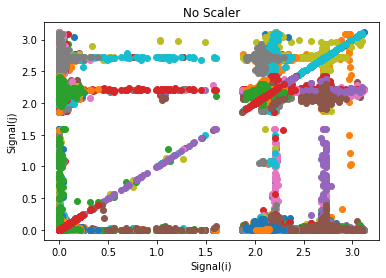
\includegraphics[scale=0.5]{noScaler.png}
	  \caption{Darstellung der Signale mit No Scaler}
	\label{noScaler}
\end{figure}

 \begin{table}[ht!]
    \begin{tabular}{|p{1.2cm}|*{9}{@{\hskip.2mm}c@{\hskip.2mm}|}}
    \hline
No Scaler &	Schranke &	Laufband &	Taster &	Band Links &	Ind. Sensor &	Licht &	Schalter &	Lichtschranke \\ \hline
count &		60300 &		60300	 &	60300 &		60300 &		60300 &		60300	 &	60300 &		60300 \\ \hline
mean &		0,356 &		0,996 &		0,01 &		0,010 &		0,022 &		1,532 &		2,044 &		0,096 \\ \hline
std &		0,916 &		1,308 &		0,138	 &	0,140 &		0,171 &		1,016 &		0,543 &		0,419 \\ \hline
min	 &	0 &		0	 &	0	 &	0 &		0 &		0 &		0 &		0 \\ \hline
25\% &		0 &		0 &		0 &		0 &		0 &		0 &		2,172 &		0 \\ \hline
50\% &		0 &		0 &		0	 &	0	 &	0	 &	2,204 &		2,198 &		0 \\ \hline
75\% &		0 &		2,720	 &	0	 &	0 &		0,016 &		2,211	 &	2,204 &		0,0161 \\ \hline
max &		3,116	 &	3,100	 &	2 &		2 &		2,224 &		2,427	 &	2,414 &		2,295 \\ \hline
    \end{tabular}
    \caption{Statistische Werte für jeden Sensor mit No Scaler}
    \label{stat}          
\end{table}

Der zweite verwendete Scaler ist der MinMaxScaler. Er skaliert den Datensatz neu, sodass alle Feature-Werte im Bereich [0, 1] liegen. Die Abbildung \ref{MinMaxScaler} repräsentiert die Daten vor und nach dem Ändern durch den Scaler. Mit Hilfe der Tabelle \ref{stat_MinMax} können wir beobachten, dass für jedes Signal die Werte jedes Punktes durch den Maximalwert jedes Signals geteilt wurden. 

\begin{figure}[ht!]
	\centering
	  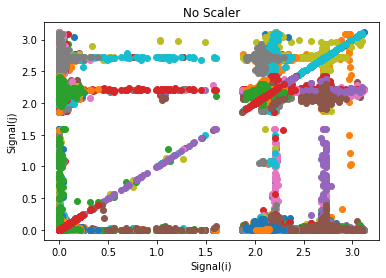
\includegraphics[scale=0.5]{noScaler.png}
	  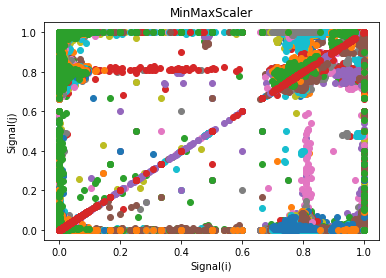
\includegraphics[scale=0.5]{MinMaxScaler.png}
	  \caption{Darstellung der Signale mit MinMaxScaler}
	\label{MinMaxScaler}
\end{figure}

 \begin{table}[ht!]
    \begin{tabular}{|p{1.2cm}|*{9}{@{\hskip.2mm}c@{\hskip.2mm}|}}
    \hline
 &	Schranke &	Laufband &	Taster &	Band Links &	Ind. Sensor &	Licht &	Schalter &	Lichtschranke \\ \hline
count &		60300 &		60300	 &	60300 &		60300 &		60300 &		60300	 &	60300 &		60300 \\ \hline
mean &		0,130 &	0,367 &	0,005 &	0,005 &	0,009 &	0,626 &	0,873 &	0,037 \\ \hline
std &		0,336 &	0,481 &	0,069 &	0,07 &	0,069 &	0,421 &	0,23 &	0,159 \\ \hline
min	 &	0 &		0	 &	0	 &	0 &		0 &		0 &		0 &		0 \\ \hline
25\% &		0 &		0 &		0 &		0 &		0 &		0 &		0,798 &		0 \\ \hline
50\% &		0 &		0 &		0	 &	0	 &	0	 &	0,81 &	0,996 &		0 \\ \hline
75\% &		0 &	1 &	0 &	0 &	0,006 &	1 &	1 &	0,006 \\ \hline
max &		1 &	1 &	1 &	1 &	1 &	1 &	1 &	1 \\ \hline
    \end{tabular}
    \caption{Statistische Werte für jeden Sensor mit MinMaxScaler}
    \label{stat_MinMax}          
\end{table}

Ein weiterer Scaler, der MinMaxScaler ähnelt, ist MaxAbsScaler. MaxAbsScaler skaliert so, dass die Trainingsdaten im Bereich liegen [-1,1] liegen, indem jeder Datenpunkt durch den Maximalwert geteilt wird. Da die Datenwerte alle positiv sind, sind die visuelle Darstellung und die statistischen Werte der Daten dieselben wie beim MinMaxScaler. Abgesehen davon, dass die beiden Scalers, wie unten gezeigt, nicht die gleichen Ergebnisse liefern.

Der nächste Scaler ist der StandardScaler. StandardScaler entfernt den Mittelwert und skaliert die Daten auf Einheitsvarianz. In der Tabelle \ref{stat_Standard} können wir sehen, dass der für jedes Signal spezifische Mittelwert nicht Null ist. Tatsächlich entfernt StandardScaler den Durchschnittswert über dem Datensatz. Wir können dies überprüfen, indem wir die Durchschnittswerte jedes Signals addieren. Wir erhalten Null (die angezeigten Werte sind gerundete Werte). Wie in Abbildung \ref{StandardScaler} zu sehen ist, hat sich bei diesem Scaler die Darstellung der Daten stark geändert, was zu erheblich anderen Ergebnissen führen kann als bei anderen Scalern mit Methoden, die Cluster verwenden. 

\begin{figure}[ht!]
	\centering
	  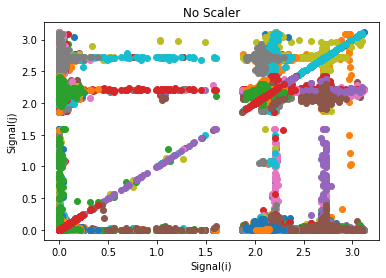
\includegraphics[scale=0.5]{noScaler.png}
	  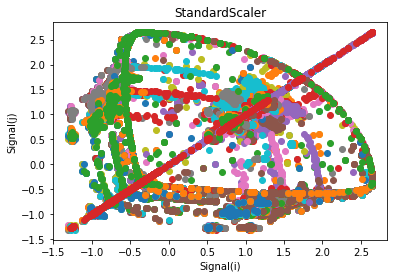
\includegraphics[scale=0.5]{StandardScaler.png}
	  \caption{Darstellung der Signale mit StandardScaler}
	\label{StandardScaler}
\end{figure}

 \begin{table}[ht!]
    \begin{tabular}{|p{1.2cm}|*{9}{@{\hskip.2mm}c@{\hskip.2mm}|}}
    \hline
 &	Schranke &	Laufband &	Taster &	Band Links &	Ind. Sensor &	Licht &	Schalter &	Lichtschranke \\ \hline
count &		60300 &		60300	 &	60300 &		60300 &		60300 &		60300	 &	60300 &		60300 \\ \hline
mean &	-0,332 &	0,227 &	-0,611 &	-0,611 &	-0,599 &	0,854 &	1,608 &	-0,535\\ \hline
std &	0,627 &	0,931 &	0,245 &	0,246 &	0,251 &	0,912 &	0,848 &	0,366\\ \hline
min &	-1,291 &	-0,979 &	-1,297 &	-1,312 &	-1,291 &	-1 &	-0,783 &	-1,291\\ \hline
25\% &	-0,581 &	-0,577 &	-0,773 &	-0,773 &	-0,761 &	-0,378 &	1,102 &	-0,758\\ \hline
50\%	 & -0,577 &	-0,378 &	-0,577 &	-0,577 &	-0,577 &	1,134 &	1,727 &	-0,577\\ \hline
75\% &	-0,378 &	1,218 &	-0,38 &	-0,38 &	-0,379 &	1,732 &	2,646 &	-0,378\\ \hline
max &	2,107 &	2,646 &	1 &	1,291 &	2,646 &	2,646 &	2,646 &	2,6456\\ \hline
    \end{tabular}
    \caption{Statistische Werte für jeden Sensor mit StandardScaler}
    \label{stat_Standard}          
\end{table}

Ein weiterer Scaler ist der RobustScaler. Die Zentrierungs- und Skalierungsstatistik vom RobustScaler basiert auf Perzentilen und wird daher nicht von einigen wenigen sehr großen Randausreißern beeinflusst. Folglich ist der resultierende Bereich der transformierten Merkmalswerte größer als bei den vorherigen Scalern, wie wir auf dem Bild \ref{RobustScaler} und in der Tabelle \ref{stat_robust} sehen können. 

\begin{figure}[ht!]
	\centering
	  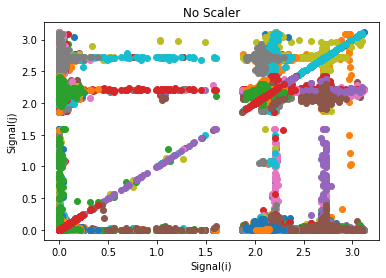
\includegraphics[scale=0.5]{noScaler.png}
	  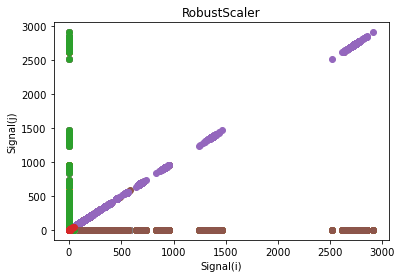
\includegraphics[scale=0.5]{RobustScaler.png}
	  \caption{Darstellung der Signale mit RobustScaler}
	\label{RobustScaler}
\end{figure}

 \begin{table}[ht!]
    \begin{tabular}{|p{1.2cm}|*{9}{@{\hskip.2mm}c@{\hskip.2mm}|}}
    \hline
 &	Schranke &	Laufband &	Taster &	Band Links &	Ind. Sensor &	Licht &	Schalter &	Lichtschranke \\ \hline
count &		60300 &		60300	 &	60300 &		60300 &		60300 &		60300	 &	60300 &		60300 \\ \hline
mean &	0,073 &	0,409 &	-0,081 &	-0,081 &	0,112 &	2,406 &	1,657 &	0,115\\ \hline
std & 	0,339 &	1,664 &	0,186 &	0,186 &	0,9 &	1,514 &	5,681 &	0,845\\ \hline
min &	-1 &	-0,5 &	-0,968 &	-0,968 &	-1 &	-0,5 &	-0,033 &	-1\\ \hline
25\% &	0 &	0 &	-0,007 &	-0,007 &	-0,001 &	0,000 &	0,987 &	0\\ \hline
50\% &	0 &	0 &	0 &	0 &	0 &	1,003 &	2,208 &	0\\ \hline
75\% &	0 &	0,709 &	0 &	0 &	0 &	4 &	4 &	0\\ \hline
max &	5,783 &	3,729 &	0,5 &	1 &	4 &	2,780 &	2912 &	44\\ \hline
    \end{tabular}
    \caption{Statistische Werte für jeden Sensor mit RobustScaler}
    \label{stat_robust}          
\end{table}

Der PowerTransformer wendet eine Leistungstransformation auf jedes Feature an, um die Daten Gauß-ähnlicher zu machen, um die Varianz zu stabilisieren und die Schiefe zu minimieren. Derzeit werden die Yeo-Johnson-Transformationen unterstützt und der optimale Skalierungsfaktor wird bei der Methode über die Maximum-Likelihood-Schätzung bestimmt. In der Abbildung \ref{PowerTransformer} ist zu sehen, dass die Verteilung der Daten dem StandardScaler ähnlich ist. Der Mittelwert der Werte aller Signale ist Null, die Werte liegen jedoch zwischen -1,293 und 2,646, wie in der Tabelle \ref{stat_power} gezeigt. 

\begin{figure}[ht!]
	\centering
	  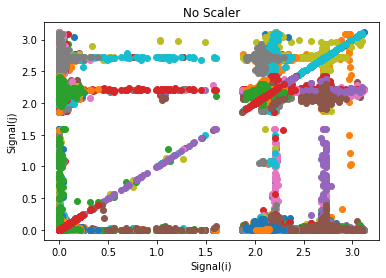
\includegraphics[scale=0.5]{noScaler.png}
	  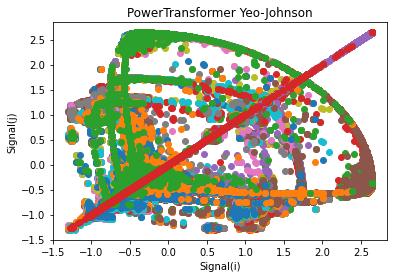
\includegraphics[scale=0.5]{PowerTransformer.png}
	  \caption{Darstellung der Signale mit PowerTransformer}
	\label{PowerTransformer}
\end{figure}

 \begin{table}[ht!]
    \begin{tabular}{|p{1.2cm}|*{9}{@{\hskip.2mm}c@{\hskip.2mm}|}}
    \hline
 &	Schranke &	Laufband &	Taster &	Band Links &	Ind. Sensor &	Licht &	Schalter &	Lichtschranke \\ \hline
count &		60300 &		60300	 &	60300 &		60300 &		60300 &		60300	 &	60300 &		60300 \\ \hline
mean &	-0,356 &	0,159 &	-0,626 &	-0,626 &	-0,587 &	0,901 &	1,655 &	-0,521\\ \hline
std &	 0,603	0,853 &	0,247 &	0,248 &	0,268 &	0,909 &	0,794 &	0,389\\ \hline
min &	-1,291 &	-0,994 &	-1,293 &	-1,307 &	-1,291 &	-1,000 &	-0,817 &	-1,291\\ \hline
25\% &	-0,602 &	-0,577 &	-0,796 &	-0,796 &	-0,748 &	-0,378 &	1,248 &	-0,737\\ \hline
50\% &	-0,577 &	-0,378 &	-0,577 &	-0,577 &	-0,577 &	1,256 &	1,732 &	-0,577\\ \hline
75\% &	-0,378 &	1,126 &	-0,405 &	-0,405 &	-0,387 &	1,732 &	2,637 &	-0,378\\ \hline
max &	1,757 &	2,630 &	1 &	1,291 &	2,646 &	2,646 &	2,646 &	2,646\\ \hline
    \end{tabular}
    \caption{Statistische Werte für jeden Sensor mit PowerTransformer}
    \label{stat_power}          
\end{table}

Der nächste Scaler ist QuantileTransformer. QuantileTransformer wendet eine nichtlineare Transformation an, sodass die Wahrscheinlichkeitsdichtefunktion jedes Merkmals auf eine gleichmäßige oder Gaußsche Verteilung abgebildet wird. QuantileTransformer wird mit zwei verschiedenen Parametern verwendet: "uniform" und "normal". Im Fall des Parameters "uniform", wie in der Abbildung \ref{uniform} und der Tabelle \ref{stat_uniform} gezeigt, liegen die Werte zwischen 0 und 1, und die Daten werden in Punkten mit denselben Abständen verteilt.

Im Fall des "normal" Parameters stellen wir in der Abbildung \ref{normal} und der Tabelle \ref{stat_normal} fest, dass dieser Scaler die Varianz innerhalb der Signale mit Werten zwischen -5,199 und 5,199 stark erhöht. 

\begin{figure}[ht!]
	\centering
	  \includegraphics[scale=0.5]{noScaler.png}
	  \includegraphics[scale=0.5]{QuantileTransformer_uniform.png}
	  \caption{Darstellung der Signale mit QuantileTransofrmer "uniform"}
	\label{uniform}
\end{figure}

 \begin{table}[ht!]
    \begin{tabular}{|p{1.2cm}|*{9}{@{\hskip.2mm}c@{\hskip.2mm}|}}
    \hline
 &	Schranke &	Laufband &	Taster &	Band Links &	Ind. Sensor &	Licht &	Schalter &	Lichtschranke \\ \hline
count &		60300 &		60300	 &	60300 &		60300 &		60300 &		60300	 &	60300 &		60300 \\ \hline
mean &	0,126 &	0,363 &	0,008 &	0,008 &	0,246 &	0,657 &	0,842 &	0,238\\ \hline
std & 	0,320 &	0,477 &	0,079 &	0,080 &	0,288 &	0,394 &	0,162 &	0,287\\ \hline
min &	0 &	0 &	0 &	0 &	0 &	0 &	0 &	0\\ \hline
25\% &	0 &	0 &	0 &	0 &	0 &	0 &	0,714 &	0\\ \hline
50\% &	0 &	0 &	0 &	0 &	0 &	0,857 &	0,857 &	0\\ \hline
75\% &	0 &	1 &	0 &	0 &	0,429 &	1 &	1 &	0,5\\ \hline
max &	1 &	1 &	1 &	1 &	1 &	1 &	1 &	1\\ \hline
    \end{tabular}
    \caption{Statistische Werte für jeden Sensor mit QuantileTransofrmer "uniform"}
    \label{stat_uniform}          
\end{table}

\begin{figure}[ht!]
	\centering
	  \includegraphics[scale=0.5]{noScaler.png}
	  \includegraphics[scale=0.5]{QuantileTransformer_normal.png}
	  \caption{Darstellung der Signale mit QuantileTransofrmer "normal"}
	\label{normal}
\end{figure}

 \begin{table}[ht!]
    \begin{tabular}{|p{1.2cm}|*{9}{@{\hskip.2mm}c@{\hskip.2mm}|}}
    \hline
 &	Schranke &	Laufband &	Taster &	Band Links &	Ind. Sensor &	Licht &	Schalter &	Lichtschranke \\ \hline
count &		60300 &		60300	 &	60300 &		60300 &		60300 &		60300	 &	60300 &		60300 \\ \hline
mean &	-4,025 &	-1,506 &	-5,117 &	-5,117 &	-2,732 &	0,514 &	2,474 &	-2,831\\ \hline
std & 	3,060 &	4,891 &	0,825 &	0,828 &	2,664 &	3,778 &	2,287 &	2,658\\ \hline
min &	-5,199 &	-5,199 &	-5,199 &	-5,199 &	-5,199 &	-5,199 &	-5,199 &	-5,199\\ \hline
25\% &	-5,199 &	-5,199 &	-5,199 &	-5,199 &	-5,199 &	-5,199 &	0,566 &	-5,199\\ \hline
50\% &	-5,199 &	-5,199 &	-5,199 &	-5,199 &	-5,199 &	1,068 &	1,068 &	-5,199\\ \hline
75\% &	-5,199 &	5,199 &	-5,199 &	-5,199 &	-0,180 &	5,199 &	5,199 &	0,000\\ \hline
max &	5,199 &	5,199 &	5,199 &	5,199 &	5,199 &	5,199 &	5,199 &	5,199\\ \hline
    \end{tabular}
    \caption{Statistische Werte für jeden Sensor mit QuantileTransofrmer "normal"}
    \label{stat_normal}          
\end{table}

Der letzte Scaler ist der Normalizer. Der Normalizer skaliert den Vektor für jede Probe neu, um unabhängig von der Verteilung der Proben eine Einheitsnorm zu erhalten. Wir beobachten aus der Abbildung \label{Normalizer} und der Tabelle \ref{stat_normalizer}, dass die Werte zwischen 0 und 0,058 verteilt sind. 

\begin{figure}[ht!]
	\centering
	  \includegraphics[scale=0.5]{noScaler.png}
	  \includegraphics[scale=0.5]{Normalizer.png}
	  \caption{Darstellung der Signale mit Normalizer}
	\label{Normalizer}
\end{figure}

 \begin{table}[ht!]
    \begin{tabular}{|p{1.2cm}|*{9}{@{\hskip.2mm}c@{\hskip.2mm}|}}
    \hline
 &	Schranke &	Laufband &	Taster &	Band Links &	Ind. Sensor &	Licht &	Schalter &	Lichtschranke \\ \hline
count &		60300 &		60300	 &	60300 &		60300 &		60300 &		60300	 &	60300 &		60300 \\ \hline
mean &	0,001 &	0,002 &	0 &	0 &	0,001 &	0,003 &	0,004 &	0,001\\ \hline
std & 	0,004 &	0,003 &	0,004 &	0,004 &	0,004 &	0,002 &	0,001 &	0,004\\ \hline
min &	0 &	0 &	0 &	0 &	0 &	0 &	0,000 &	0\\ \hline
25\% &	0 &	0 &	0 &	0 &	0 &	0 &	0,004 &	0\\ \hline
50\% &	0 &	0 &	0 &	0 &	0 &	0,005 &	0,004 &	0\\ \hline
75\% &	0 &	0,007 &	0 &	0 &	0 &	0,005 &	0,004 &	0\\ \hline
max &	0,013 &	0,008 &	0,059 &	0,058 &	0,053 &	0,005 &	0,005 &	0,022\\ \hline
    \end{tabular}
    \caption{Statistische Werte für jeden Sensor mit Normalizer}
    \label{stat_normalizer}          
\end{table}

\clearpage

Unter diesen Scalern werden nur No Scaler, BooleanScaler, MinMaxScaler und StandardScaler angewendet, da für jeden Scaler die neuronalen Netze für jede Fenstergröße neu trainiert werden müssen.

Für die DBSCAN-Methode werden No Scaler, MinMaxScaler, StandardScaler und RobustScaler angewendet. Scalern wie BooleanScaler funktionieren nicht für DBSCAN, da die Verteilung von Daten für diese Art von Scaler keinen einzelnen Cluster ergeben kann, dessen normales Verhalten vorliegt.

Für die SVM- und LOF-Methoden werden alle Scaler verwendet. 

\subsection{Training}

Die auf neuronalen Netzen basierenden Methoden werden über zehn Epochen trainiert, da sie schnell ihren minimalen Loss erreichen, wie in Abbildung \label{loss} gezeigt. Diese Methoden werden auch auf eine kleine Anzahl von Methoden trainiert, um eine Überanpassung zu vermeiden. Für diese beiden Modelle wird als Kostenfunktion der Root Mean Square Error (RMSE) verwendet. 

 \begin{figure}[ht!]
	\centering
	  \includegraphics[scale=0.5]{evol_1DCNN.png}
	  \includegraphics[scale=0.5]{loss_Autoencoder.png}
	  \caption{Loss Evolution für 1DCNN (links) und Autoencoder (rechts)}
	\label{loss}
\end{figure}

Methoden, die Cluster verwenden, haben eine Trainingsphase in der sie die Normalverhalten über eine Epoch lernen. Um eine Anomalieerkennung durchzuführen, wird jeder Test- und Angriff-Datensatz den Cluster-Methoden mit dem Trainingsdatensatz übergeben. 

\subsection{Evaluation Methode}

Bei 1DCNN und Autoencoder werden die Daten am Ausgang der neuronalen Netze mit den realen Daten verglichen. Für beide Methoden wurden für jeden Datenpunkt ein Schwellenwert verwendet, um zu entscheiden, ob eine Anomalie vorliegt. Wenn der Unterschied zwischen den Daten kleiner als der Schwellenwert ist, liegt keine Anomalie vor, da sonst eine Anomalie festgestellt wurde. Diese Methode wird als Punkt-Classifier bezeichnet. Jeder Datenpunkt wird dann einzeln mit einem Fenster verglichen, in dem jeder Punkt beschriftet wurde.

Ebenso wird für die SVM-, LOF- und DBSCAN-Methoden das Ergebnis mit einem Array verglichen, sodass jeder Punkt beschriftet wurde.

Für Autoencoder wurde eine andere Auswertungsmethode verwendet, die darauf abzielt, das gesamte Fenster als Ausgabe des neuronalen Netzwerks zu klassifizieren. Diese Methode wird als Fenster Classifier bezeichnet. Um abzuschätzen, ob das Fenster eine Anomalie aufweist, wird der RMSE im Fenster berechnet und das Ergebnis mit einem Schwellenwert verglichen. Wenn das Ergebnis unter dem Schwellenwert liegt, befindet sich ebenfalls keine Anomalie im Fenster, andernfalls wird eine Anomalie erkannt. Das Ergebnis wird dann mit einem beschrifteten Fenster verglichen.

Um dann die Leistung jeder Methode abzuschätzen, werden die Methoden über ihre Accuracy, Precision, Recall und $ F_{1}$-Maß bewertet. Wir müssen zuerst die Begriffe True Positive, True Negative, False Positive und False Negative in der Anomalieerkennung definieren.

True Positive (TP) ist, wenn das Modell eine Anomalie erkennt und derzeit eine Anomalie vorliegt.

True Negative (TN) ist, wenn das Modell keine Anomalie erkennt, d.h. es erkennt normales Verhalten und derzeit gibt es keine Anomalie.

False Positive (FP) ist, wenn das Modell eine Anomalie erkennt, während derzeit keine Anomalie vorliegt.

False Negative (FN) ist, wenn das Modell keine Anomalie erkennt, während eine Anomalie vorliegt.

Diese Daten werden erhalten, indem verglichen wird, was das Modell mit der Ground Truth erkannt hat. Die Ground Truth ist ein beschriftetes Array, in dem angezeigt wird, ob ein normales Verhalten oder eine Anomalie vorliegt. Für die 1DCNN- und Autoencoder- Modell mit dem Punkt Classifier vergleichen wir nach dem Vergleich der Daten Punkt für Punkt in dem Output der Modelle mit den aktuellen Daten und nachdem wir dank des Schwellenwerts entschieden haben, ob eine Anomalie vorliegt oder nicht, mit dem Ground Truth, ein Array, das für jeden Datenpunkt angibt, ob eine Anomalie oder ein normales Verhalten vorliegt. Für den Fenster Classifier ist die Ground Truth ein Array, das für jedes Fenster angibt, ob ein normales Verhalten oder eine Anomalie vorliegt.

Bei SVM-, LOF- und DBSCAN-Modellen werden die Output Daten genau wie beim Punkt Classifier, Punkt für Punkt mit der Ground Truth verglichen.  

Accuracy, Precision, Recall und $ F_{1}$-Maß werden wie folgt definiert: 

\begin{align}
 	Accuracy = \frac{TP + TN}{Alle\_Daten} \\
	Precision = \frac{TP}{TP + FP} \\
	Recall = \frac{TP}{TP + FN} \\
	F_{1} = 2 \cdot \frac{Precision \cdot Recall}{Precision + Recall} 
\end{align}

Die Accuracy gibt daher im Allgemeinen an, wie gut die Erkennung von Anomalien und normalem Verhalten ist. Die Precision gibt an, ob viele falsche Anomalien gemeldet wurden. Der Recall zeigt an, ob das Modell bei einer Anomalie häufig ein normales Verhalten festgestellt hat. Die $ F_{1}$-Maß gibt einen allgemeinen Hinweis auf die Leistung des Modells. \\

Zunächst werden die Ergebnisse für jedes Modell mit jeder Hyperparameter Tuning dargestellt. Für jedes Modell wurde die Evaluation in zwei Szenarien aufgeteilt. Das erste Szenario ist die Erkennung eines normalen Verhaltens dank des Testdatensatzes. Das zweite Szenario ist die Erkennung von Anomalien mit Angriffsdatensätzen. \\

\subsection{1DCNN}

Für die 1DCNN-Methode wurde das Modell mit den Fenstergrößen 5, 10, 20, 33, 66 trainiert. Zusätzlich wurden für diese fünf Modelle die Scaler No Scaler, BooleanScaler, MinMaxScaler und StandardScaler verwendet. Dies macht insgesamt 20 verschiedene Modelle, die trainiert wurden. Hier wird nur das Modell vorgestellt, für das die Fenstergröße das beste Ergebnis liefert. Für jedes Modell wurde der Mittelwert jeder Bewertungsmethode (Accuracy, Precision, Recall, $F_{1}$-Maß) jedes Signals berechnet und aufgezeichnet.

Die besten Ergebnisse werden bei einer Fenstergröße von 20 erzielt. In der Abbildung \ref{1DCNN_20} ist die Entwicklung der Erkennung von Anomalien und normalen Verhaltensweisen in Bezug auf den Schwellenwert dargestellt. Es wird für jedes Modell beobachtet, dass je mehr der Wert des Schwellenwerts zunimmt, desto mehr die Anomalieerkennung abnimmt und die Erkennung normaler Verhaltens zunimmt. Dies ist normal, da durch Erhöhen des Schwellenwerts die Differenz zwischen den Ausgabewerten des Modells und den aktuellen Werten erhöht werden kann, ohne dass dies als Anomalie erkannt wird. Umgekehrt wird bei einem niedrigen Schwellenwert eine niedrige Wertabweichung als Anomalie erkannt.

Wir beobachten, dass die Angriff Accuracy zwischen 40 und 65 Prozent für eine Accuracy des Testdatensatzes zwischen 0 und 99 Prozent variiert. 

\begin{figure}[ht!]
	\centering
	  \includegraphics[scale=0.5]{1DCNN_20.png}
	  \caption{1D CNN mit Fenster Größe 20 Test und Angriff Accuracy}
	\label{1DCNN_20}
\end{figure}

In der Abbildung \ref{sis_1DCNN_20} ist die Entwicklung der Erkennung des Safety Angriff im Vergleich zum Schwellenwert dargestellt. Es wird beobachtet, dass die Anomalieerkennung für Safety Angriff für einen niedrigen Schwellenwert hoch ist. Bei diesem Angriff muss jedoch keine Anomalie erkannt werden, da dieser Angriff das normale Verhalten des Prozesses nicht verändert. Daher wird eher eine geringe Accuracy bevorzugt. 

\begin{figure}[ht!]
	\centering
	  \includegraphics[scale=0.5]{sis_1DCNN_20.png}
	  \caption{1D CNN mit Fenster Größe 20 Safety Angriff Accuracy}
	\label{sis_1DCNN_20}
\end{figure}

Von allen Fenstergrößen ist die Größe 20 diejenige, die die besten Ergebnisse liefert. Unter den verschiedenen Scalern für diese Fenstergröße ist die StandardScaler diejenige, die die besten Ergebnisse liefert. Bei einem Schwellenwert von 0,25 beträgt die Accuracy des Testdatensatzes 65 Prozent, bei einer Angriff Accuracy von 63 Prozent und einer Safety Angriff Accuracy von 34 Prozent. 

\subsection{Autoencoder}

Für die Autoencoder-Methode wurde das Modell für eine einzelne Fenstergröße in Eingabe: 40 Datenpunkte trainiert. Es wurden zwei Entscheidungsmethoden verwendet: Punkt Classifier und Fenster Classifier. Für diese beiden wurden Methoden die Scaler No Scaler, Boolean Scalers und MinMaxScaler und StandardScaler verwendet. Für jedes Modell wurde der Mittelwert jeder Bewertungsmethode (Accuracy, Precision, Recall, $F_{1}$-Maß) jedes Signals berechnet und aufgezeichnet.

Die Ergebnisse für den Punkt Classifier sind in Abbildung \ref{autoencoder_40} dargestellt. Wir beobachten Diagramme ähnlich den Diagrammen der 1DCNN-Modelle. Die Accuracy des Testdatensatzes nimmt mit zunehmendem Schwellenwert und abnehmender Precision und Recall von Angriffen zu. Die Angriff Accuracy weicht jedoch kaum von der 50 Prozent Schwelle ab. Die Safety Angriff Accuracy liegt zwischen 47 und 58 Prozent für eine Test Accuracy zwischen 0 und 99 Prozent. Wie 1DCNN kann der Test Accuracy hohe Werte erreichen, aber die Angriff Accuracy ist niedriger als beim 1DCNN-Modell. 

\begin{figure}[ht!]
	\centering
	  \includegraphics[scale=0.5]{autoencoder_40.png}
	  \caption{Autoencoder Punkt Classifier Test und Angriff Accuracy}
	\label{autoencoder_40}
\end{figure}

In der Abbildung \ref{autoencoder_40_classifier} sind die Ergebnisse dargestellt, die mit dem Fenster Classifier für das Modell erhalten wurden. Die Ergebnisse sind hinsichtlich der Erkennungsanomalie ähnlich wie bei den Modellen, die den Punkt Classifier verwenden. Bei Scaler wie MinMaxScaler und StandardScaler für die Klassifizierungsmethode, Fentser Classifier, ist die Erkennung normaler Verhaltensweisen jedoch schwächer. 

\begin{figure}[ht!]
	\centering
	  \includegraphics[scale=0.5]{autoencoder_40_classifier.png}
	  \caption{Autoencoder Window Classifier Test und Angriff Accuracy}
	\label{autoencoder_40_classifier}
\end{figure}

In der Abbildung \ref{sis_autoencoder} ist die Accuracy für Safety Angriff Accuracy für beide Klassifizierungsmethode dargestellt. Man kann beobachten, dass sich alle Scalern für den Fenster Classifier viel schneller Null nähern als für den Punkt Classifier. Bei einem Schwellenwert von mehr als 0,5 haben alle Scaler eine Accuracy für Safety Angriff Accuracy nahe Null. 

\begin{figure}[ht!]
	\centering
	  \includegraphics[scale=0.5]{sis_autoencoder_40.png}
	  \includegraphics[scale=0.51]{sis_autoencoder_40_classifier.png}
	  \caption{Autoencoder Punkt Classifier (links) und Fenster Classifier (rechts) Safety Angriff Accuracy}
	\label{sis_autoencoder}
\end{figure}

Von den beiden Klassifizierungsmethoden liefert der Punkt Classifier bessere Ergebnisse für die Erkennung von Anomalien und normalem Verhalten. Mit dem MinMaxScaler und einem Schwellenwert von 0,25 beträgt die Angriff Accuracy 58 Prozent bei einer normalen Verhalten Accuracy von 86 Prozent bei einer Safety Angriff Accuracy von 15 Prozent. 

\subsection{SVM}

Für die SVM-Methode muss das Modell nur über eine Epoche trainiert werden. Wir verwenden den Trainingsdatensatz als Referenz für alle anderen Datensätze. In der Ausgabe des Modells befindet sich ein Array von 1 und -1, wobei 1 ein normales Verhalten und -1 eine Anomalie bedeutet. Im Gegensatz zu früheren Modellen gibt es kein spezifisches Ergebnis für jedes Signal im Prozess. Jeder Punkt wird mit dem entsprechenden Punkt eines beschrifteten Arrays verglichen. Für dieses Modell werden alle Scaler verwendet. Für jeden Scaler wurden mehrere Werte für den "Nu" -Parameter verwendet: 0,01, 0,1, 0,25, 0,5, 0,75 und 0,9. 

Die Ergebnisse der einzelnen Scaler sind in Abbildung \ref{svm_results} dargestellt. Für jeden Scaler werden unterschiedliche Ergebnisse erhalten. Wir beobachten für einen großen Teil der Scaler jedoch, dass die Genauigkeit des Testdatensatzes umso mehr abnimmt, je mehr der Wert von "Nu" zunimmt. Ebenso ändert sich die Angriffsgenauigkeit im Vergleich zu den Werten von "Nu" kaum. 

Bei StandardScaler und PowerTransformer überschreitet der Test Accuracy 70 Prozent nicht. Die Angriff Accuracy für diese beiden Scaler liegt zwischen 40 und 70 Prozent.

Für die beiden QuantileTransformers sind die Ergebnisse mit einer Angriff Accuracy von maximal 60 Prozent und einer Test Accuracy von 99 Prozent sehr ähnlich.

Die besten Ergebnisse für die Angriff Accuracy werden für MinMaxScaler, MaxAbsScaler, BooleanScaler und Normalizer erzielt, mit denen bis zu 70 Prozent erzielt werden konnte. 

\begin{figure}[ht!]
	\centering
	  \includegraphics[scale=0.5]{svm_1.png}
	  \includegraphics[scale=0.5]{svm_2.png}
	  \includegraphics[scale=0.5]{svm_3.png}
	  \caption{SVM Test und Angriff Accuracy}
	\label{svm_results}
\end{figure}

In der Abbildung \ref{sis_svm_results} sind die Ergebnisse für die Accuracy des Safety Angriff dargestellt. Wir beobachten, dass bei allen Scalern die Accuracy zunimmt, wenn der Wert des Parameters "Nu" erhöht wird. Die RobustScaler, StandardScaler, MinMaxScaler und PowerTransformer weisen eine zu hohe Accuracy auf, als dass sie für das SVM-Modell verwendet werden könnten. 

\begin{figure}[ht!]
	\centering
	  \includegraphics[scale=0.5]{sis_svm_1.png}
	  \includegraphics[scale=0.5]{sis_svm_2.png}
	  \includegraphics[scale=0.5]{sis_svm_3.png}
	  \caption{SVM Safety Angriff Accuracy}
	\label{sis_svm_results}
\end{figure}

Die besten Ergebnisse werden für den Scaler Normalizer bei einem Wert des Parameters "Nu" von 0,1 erzielt. Der Test Accuracy beträgt 91 Prozent bei einer Angriff Accuracy von 62 Prozent und Safety Angriff von 1 Prozent. 

\subsection{LOF}

Wie das SVM-Modell wird auch das LOF-Modell über eine Epoche trainiert. Der Trainingsdatensatz dient als Referenz für normales Verhalten. Alle Scaler werden für die LOF-Methode verwendet. Bei dem Input des Modells wird zunächst der Trainingsdatensatz angegeben, damit das Modell das normale Verhalten des Prozesses lernt. Das Modell erhält dann den Datensatz, anhand dessen das normale Verhalten oder die Anomalie erkannt wird. In der Ausgabe gibt das LOF-Modell genau wie das SVM-Modell ein Array von 1 und -1 an, wobei 1 für normales Verhalten und -1 für eine Anomalie steht. Für jeden Scaler wurden unterschiedliche Nachbar-Werte verwendet: 5, 20, 100, 500, 1000 und 2000.

Die Ergebnisse für das LOF-Modell sind in Abbildung \ref{lof_results} dargestellt. Es wird beobachtet, dass für den StandardScaler, den RobustScaler, den MinMaxScaler, den MaxAbsScaler und den PowerTransformer der Test Accuracy unter 60 Prozent liegt. Diese Methoden können daher nicht für das LOF-Modell verwendet werden.

\begin{figure}[ht!]
	\centering
	  \includegraphics[scale=0.5]{lof_1.png}
	  \includegraphics[scale=0.5]{lof_2.png}
	  \includegraphics[scale=0.5]{lof_3.png}
	  \caption{LOF Test und Angriff Accuracy}
	\label{lof_results}
\end{figure}

Bei No Scaler, BooleanScaler und Normalizer nimmt der Test Accuracy mit zunehmender Anzahl der Nachbarn ab. Umgekehrt erhöht sich bei den beiden QuantileTransformer-Methoden der Test Accuracy, wenn die Anzahl der Nachbarn zunimmt. 

In der Abbildung \ref{sis_lof_results} sind die Ergebnisse für Safety Angriff dargestellt. Wir stellen fest, dass für den StandardScaler, den MinMaxScaer, den MaxAbsScaler, den RobustScaler und den PowerTransofrmer die Accuracy des Safety Angriff Accuracy viel zu hoch ist, da dieser Angriff das normale Verhalten des Prozesses nicht verändert und das Modell keine Anomalie erkennen darf so dass die Accuracy nahe Null sein muss.

Der BooleanScaler hat für dieses Modell eine Safety Angriff Accuracy von nahezu Null.

Wir stellen fest, dass bei den beiden QuantileTransformern die Accuracy abnimmt, wenn die Anzahl der Nachbarn zunimmt. 

\begin{figure}[ht!]
	\centering
	  \includegraphics[scale=0.45]{sis_lof_1.png}
	  \includegraphics[scale=0.45]{sis_lof_2.png}
	  \includegraphics[scale=0.45]{sis_lof_3.png}
	  \caption{LOF Safety Angriff Accuracy}
	\label{sis_lof_results}
\end{figure}

Für das LOF-Modell werden die besten Ergebnisse für den No Scaler mit einer Anzahl von Nachbarn von 5 erzielt. Für diese Parameterwerte beträgt der Test Accuracy 92 Prozent für eine Angriff Accuracy von 63 Prozent und eine Safety Angriff Accuracy von 5 Prozent. 

\subsection{DBSCAN}

DBSCAN hat wie die beiden vorherigen Modelle eine Lernphase mit nur eine Epoche und verwendet den Trainingsdatensatz als Referenz für normales Verhalten. Die verwendeten Scaler sind No Scaler, MinMaxScaler, RobustScaler und StandardScaler. Bei dem Input des Modells wird zunächst der Trainingsdatensatz angegeben, damit das Modell das normale Verhalten des Prozesses lernt. Das Modell erhält dann den Datensatz, anhand dessen das normale Verhalten oder die Anomalie erkannt wird. In der Ausgabe gibt das DBSCAN-Modell ein Array mit einer Zahl größer oder gleich -1 an. Wenn sich die Zahl von -1 unterscheidet, entspricht dies einem Cluster mit normalem Verhalten. Im Idealfall sollte das Modell nur einen Cluster mit der Nummer 0 angeben. Wenn die Nummer -1 ist, wurde eine Anomalie festgestellt. Das DBSCAN-Modell wurde auf unterschiedliche Werte von "eps" der den maximalen Abstand zwischen zwei Samples darstellen, damit sie in demselben Sample berücksichtigt werden und mit dem Parameter "min\_samp", welches die maximale Anzahl von Samples in einer Nachbarschaft darstellt, damit dies als Kernpunkt betrachtet wird.

Für DBSCAN experimentierte ich mit dem Parameter, der den maximalen Abstand zwischen zwei Samples darstellen, damit sie in demselben Sample berücksichtigt werden, und mit dem Parameter, welches die maximale Anzahl von Samples in einer Nachbarschaft darstellt, damit dies als Kernpunkt betrachtet wird. Diese beiden Parameter wurden so gewählt, dass DBSCAN ein einzelnes Cluster erkennt, wobei der eine das normale Verhalten des Prozesses neu gruppiert und alle Ausreißer die Punkte sind, die eine Anomalie erkennen.

In der Abbildung \ref{dbscan_results} sind die Ergebnisse des Test Accuracy und Angriff Accuracy für das DBSCAN-Modell dargestellt. Wir beobachten für alle Scaler hohe Werte für den Angriff Accuracy von bis zu 74 Prozent und bis zu 99 Prozent für den Testdatensatz, der nur normales Verhalten enthält. 

\begin{figure}[ht!]
	\centering
	  \includegraphics[scale=0.5]{dbscan_4.png}
	  \caption{DBSCAN Test und Angriff Accuracy}
	\label{dbscan_results}
\end{figure}

In der Abbildung \ref{sis_dbscan_results} sind die Ergebnisse für den Safety Angriff dargestellt. Wir stellen fest, dass die Accuracy im Allgemeinen nahe Null liegt, außer im Fall des No Scaler für die Parameter $eps = 1,2$ und $min\_samp = 20.000$, von denen die Accuracy 100 Prozent beträgt. Für diesen Scaler und diese Parameterwerte ist das Modell also nicht realisierbar. 

\begin{figure}[ht!]
	\centering
	  \includegraphics[scale=0.45]{sis_dbscan_4.png}
	  \caption{DBSCAN Safety Angriff Accuracy}
	\label{sis_dbscan_results}
\end{figure}

Die besten Ergebnisse werden daher für den MinMaxScaler mit den Parametern $eps = 0.6003$ und $min\_samp = 15000$ erzielt. Der Test Accuracy beträgt 88 Prozent, die Angriff Accuracy 65 Prozent und die Safety Angriff Accuracy 15 Prozent. 

\subsection{Diskussion}

Nach Analyse der für jedes Modell, jeden Scaler und jeden Hyperparameter erhaltenen Ergebnisse konnten die besten Ergebnisse für jedes Modell ermittelt werden. In der Abbildung \ref{ergebnis} sind die besten Ergebnisse jedes Modells gruppiert, d.h. DBSCAN mit dem MinMaxScaler für die Parameter $eps = 0,6003$ und $min\_samp = 15000$, SVM mit dem Normalisierer und $nu = 0,1$, LOF mit dem No Scaler und einer Anzahl von Nachbarn gleich 5, 1DCNN mit dem StandardScaler, dem Schwellenwert gleich 0,25 und einem Input Fenster der Größe 20 und Autoencder mit dem MinMaxScaler, dem Punkt Classifier und einem Schwellenwert gleich 0,25. 

\begin{figure}[ht!]
	\centering
	  \includegraphics[scale=0.7]{ergebnis.png}
	  \caption{Ergebnisse}
	\label{ergebnis}
\end{figure}

Wir stellen fest, dass das LOF-Modell mit 92 Prozent die beste Accuracy für Testdatensätze bietet. DBSCAN hat mit 65 Prozent die beste Angriffs Accuracy. Das SVM-Modell hat die höchste Precision mit 77 Prozent und die niedrigste Accuracy für Safety Angriff Accuracy mit 1 Prozent. 1DCNN hat den höchsten Recall mit 63 Prozent und den höchsten $F_{1}$-Maß mit 56 Prozent, aber die schlechteste Accuracy für Safety Angriff Accuracy mit 34 Prozent. 

Es wird daher beobachtet, dass die Methoden, die Cluster verwenden und keine neuronalen Netze verwenden, bessere Ergebnisse für die Erkennung von normalem Verhalten und die Erkennung von Anomalien liefern. DBSCAN mit dem MinMaxScaler für die Parameter $eps = 0.6003$ und $min\_samp = 15000$ ist daher das beste Modell. 

%%%%%%%%%%%%%%%%%%%%%%%%%%%%%%%%%
 \newpage  % neuer Abschnitt auf neue Seite, kann auch entfallen
%%%%%%%%%%%%%%%%%%%%%%%%%%%%%%%%%

\section{Erkenntnis}


In dieser Masterarbeit konnte ich die Signale eines Prozesses mithilfe der Raspberry Pi 3 erfassen, mit dem Objekte nach ihrer Beschaffenheit sortiert wurden. Das Basiskabel, das den Bukoppler mit dem Prozess verbindet, wurde durch einen Y-Schalter ersetzt. Die Spannung vom System wurde mit einer Spannung Reduktion Montage reduziert, um elektronische Komponenten wie den Raspberry zu schützen. Mit diesen Signalen habe ich sie in zwei Datensätze unterteilt, einen Trainingsdatensatz und einen Testdatensatz. Aus den über die Raspberry aufgezeichneten Angriffen wurden Angriffsdatensätze erstellt. Die Datensätze wurden mit Scalern erstellt, um die Abhängigkeit von Lernmodellen von Scalern zu beobachten. Fünf Methoden wurden verwendet: CNN, Autoencoder, SVM, LOF, DBSCAN. Jedes Modell wurde über Hyperparamter Tuning optimiert, immer mit dem Ziel, die besten Ergebnisse zu erzielen.  DBSCAN liefert uns die besten Ergebnisse.

Diese Ergebnisse könnten verbessert werden, indem die Anomalie auf jedem einzelnen Sensor erkannt wird oder indem bessere Methoden zur Schwellenwertauswahl angewendet werden. Zur Vorbereitung der Daten können andere Methoden als Scalern verwendet werden, z.B. PCA oder maschinelles Lernen.

Anschließend wäre es interessant, das Modell an verschiedenen Prozessen mit einer größeren Anzahl von Signalen oder Angriffen zu testen. Es könnte auch interessant sein, die Erkennung von Anomalien auf den Signalen unabhängig zu analysieren, da einige Angriffe auf bestimmte Signale leichter sind als auf andere. Weitere Arbeiten zur Erkennung von Anomalien in Echtzeit können durchgeführt werden, um festzustellen, ob das Modell schnell genug ist, um eine Anomalie zu erkennen.



%%%%%%%%%%%%%%%%%%%%%%%%%%%%%%%%%
 \newpage  % neuer Abschnitt auf neue Seite, kann auch entfallen
%%%%%%%%%%%%%%%%%%%%%%%%%%%%%%%%%
\section*{Anhang}
\thispagestyle{plain}

\begin{figure}[ht!]
	\centering
	  \includegraphics[scale=0.5]{noScaler.png}
	  \includegraphics[scale=0.5]{MaxAbsScaler.png}
	  \caption{Darstellung der Signale mit MinMaxScaler}
\end{figure}

\thispagestyle{plain}

 \begin{table}[ht!]
    \begin{tabular}{|p{1.2cm}|*{9}{@{\hskip.2mm}c@{\hskip.2mm}|}}
    \hline
 &	Schranke &	Laufband &	Taster &	Band Links &	Ind. Sensor &	Licht &	Schalter &	Lichtschranke \\ \hline
count &		60300 &		60300	 &	60300 &		60300 &		60300 &		60300	 &	60300 &		60300 \\ \hline
mean &	0,130 &	0,367 &	0,005 &	0,005 &	0,009 &	0,626 &	0,873 &	0,037\\ \hline
std &	0,336 &	0,481 &	0,069 &	0,070 &	0,069 &	0,421 &	0,230 &	0,159\\ \hline
min &	0 &	0 &	0 &	0 &	0 &	0 &	0 &	0\\ \hline
25\% &	0 &	0 &	0, &	0 &	0 &	0 &	0,798 &	0\\ \hline
50\% &	0 &	0 &	0 &	0 &	0 &	0,810 &	0,996 &	0\\ \hline
75\% &	0 &	1 &	0 &	0 &	0,006 &	1 &	1 &	0,006\\ \hline
max &	1 &	1 &	1 &	1 &	1 &	1 &	1 &	1\\ \hline
    \end{tabular}
    \caption{Statistische Werte für jeden Sensor mit MinMaxScaler}
    \label{stat_MinMaxScaler}          
\end{table}

 \newpage
\thispagestyle{plain}

\begin{figure}[ht!]
	\centering
	  \includegraphics[scale=0.5]{1DCNN_5.png}
	  \caption{1D CNN mit Fenster Größe 5}
	\label{1DCNN_20}
\end{figure}

\thispagestyle{plain}

\begin{figure}[ht!]
	\centering
	  \includegraphics[scale=0.5]{1DCNN_10.png}
	  \caption{1D CNN mit Fenster Größe 10}
	\label{1DCNN_20}
\end{figure}
 \newpage
\thispagestyle{plain}

\begin{figure}[ht!]
	\centering
	  \includegraphics[scale=0.5]{1DCNN_33.png}
	  \caption{1D CNN mit Fenster Größe 33}
	\label{1DCNN_20}
\end{figure}

\thispagestyle{plain}

\begin{figure}[ht!]
	\centering
	  \includegraphics[scale=0.5]{1DCNN_66.png}
	  \caption{1D CNN mit Fenster Größe 66}
	\label{1DCNN_20}
\end{figure}
 \newpage
\thispagestyle{plain}

\begin{figure}[ht!]
	\centering
	  \includegraphics[scale=0.5]{sis_1DCNN_5.png}
	  \includegraphics[scale=0.5]{sis_1DCNN_10.png}
	  \includegraphics[scale=0.5]{sis_1DCNN_33.png}
	  \includegraphics[scale=0.5]{sis_1DCNN_66.png}
	  \caption{Safety Angriff 1D CNN mit Fenster Größe 5 (oben links), 10 (oben rechts), 33 (unten links) und 66 (unten rechts)}
	\label{1DCNN_20}
\end{figure}

\thispagestyle{plain}
 \newpage
\clearpage

\thispagestyle{plain}

%%%%%%%%%%%%%%%%%%%%%%%%%%%%%%%%%
 \newpage  % neuer Abschnitt auf neue Seite, kann auch entfallen
%%%%%%%%%%%%%%%%%%%%%%%%%%%%%%%%%
\section*{Quellen}

\thispagestyle{plain}

\noindent [1] Deng L , Yu D . Deep learning: methods and applications[J]. Foundations \& Trends in Signal Processing, 2014, 7(3):197-387. \\

\noindent [2] 	Grohmann, J.; Herbst, N.; Chalbani, A.; Arian, Y.; Peretz, N.; Kounev, S. A Taxonomy of Techniques for SLO Failure Prediction in Software Systems. Computers 2020, 9, 10. https://doi.org/10.3390/computers9010010 \\

\noindent [3]	 Yangdong He and Jiabao Zhao, “Temporal Convolutional Networks for Anomaly Detection in Time Series”, 2019 J. Phys.: Conf. Ser. 1213 042050 \\

\noindent [4] 	Verma, K., Gupta, V., Sharma, M., \& Sevakula, R. (2013). Intelligent condition based monitoring of rotating machines using sparse auto-encoders. IEEE

\noindent [5]	 K. K. Reddy, S. Sarkar, V. Venugopalan, and M. Giering, “Anomaly Detection and Fault Disambiguation in Large Flight Data: A Multi-modal Deep Auto-encoder Approach.” in Annual Conf. Prognostics and Health Management Society (2016). \\

\noindent [6] 	V. T. Tran, H. T. Pham, B. S. Yang, and T. T. Nguyen, “Machine performance degradation assessment and remaining useful life prediction using proportional hazard model and support vector machine.” Mechanical Syst. Signal Process., 32, 320 (2012). \\

\noindent [7] 	Credit Card Fraud Detection: Neural Network vs. Anomaly Detection Algorithms, Harsh Bansal, https://medium.com/analytics-vidhya/credit-card-fraud-detection-c66d1399c0b7 \\

\noindent [8] 	Scikit-learn: Machine Learning in Python, Pedregosa, F. and Varoquaux, G. and Gramfort, A. and Michel, V.and Thirion, B. and Grisel, O. and Blondel, M. and Prettenhofer, P. and Weiss, R. and Dubourg, V. and Vanderplas, J. and Passos, A. and Cournapeau, D. and Brucher, M. and Perrot, M. and Duchesnay, E., Journal of Machine Learning Research, volume 12, pages 2825-283, 2011 \\








\end{document}

